% aliveKat
\documentclass[aps,pra,superscriptaddress,reprint,nofootinbib]{revtex4-1}
% \documentclass[prb,reprint,nofootinbib]{revtex4-1} 
% \documentclass[pra,superscriptaddress,reprint,nofootinbib]{revtex4-1}
% \documentclass[prb,preprint,letterpaper,noeprint,longbibliography,nodoi,footinbib]{revtex4-1} 


% worry about formatting AFTER the text is written


\usepackage[utf8]{inputenc}
\usepackage{amsmath,amssymb,amsthm}
\usepackage{amsfonts}
\usepackage{graphicx}
\usepackage{float}
\usepackage{mathtools}
\usepackage[usenames,dvipsnames]{xcolor}	
\usepackage{hyperref}
% \usepackage{siunitx}
\usepackage{textcomp}
\usepackage{subfiles}
\usepackage{comment}
% \usepackage[bottom]{footmisc}
% \usepackage{subfig}
% \usepackage[style=base]{caption}
\usepackage{subfig}

\usepackage{silence}
\WarningFilter{revtex4-1}{Repair the float}

%\bibliographystyle{apsrev4-2}
%\setlength{\parindent}{0pt}

\newcommand{\abs}[1]{\left\lvert #1 \right\rvert}
\newcommand{\norm}[1]{\left\lVert #1 \right\rVert}
\newcommand{\ip}[2]{\langle #1,#2 \rangle}
\newcommand{\expect}[1]{\langle #1 \rangle}

\newcommand{\code}[1]{\texttt{#1}}
\newcommand{\jam}[1]{\textcolor{magenta}{\textbf{#1}}}


\begin{document}
\title{Optical modelling of advanced gravitational wave detector configurations}

\author{James W. Gardner}
\email{u6069809@anu.edu.au}
\affiliation{College of Science, Australian National University, Acton, ACT, 2601, Australia}

\author{Vaishali B. Adya}
% \email{vaishali.adya@anu.edu.au}
\affiliation{Centre for Gravitational Astrophysics, The Australian National University, Acton, A.C.T., 2601, Australia}
\affiliation{OzGrav @ ANU, Australian Research Council Centre of Excellence for Gravitational Wave Discovery, Acton, A.C.T., 2601, Australia}

\author{David McClelland}
% \email{david.mcclelland@anu.edu.au}
\affiliation{Centre for Gravitational Astrophysics, The Australian National University, Acton, A.C.T., 2601, Australia}
\affiliation{OzGrav @ ANU, Australian Research Council Centre of Excellence for Gravitational Wave Discovery, Acton, A.C.T., 2601, Australia}

\author{Daniel Töyrä}
% \email{daniel.toyra@anu.edu.au}
\affiliation{Centre for Gravitational Astrophysics, The Australian National University, Acton, A.C.T., 2601, Australia}
\affiliation{OzGrav @ ANU, Australian Research Council Centre of Excellence for Gravitational Wave Discovery, Acton, A.C.T., 2601, Australia}

\date{\today}


%%%%%%%%%%%%%%%%%%%%%%%%%%%%%%%%%%%%%%%%%%
\begin{abstract}
% single paragraph, short sales pitch

Gravitational wave detectors are highly complex and their transfer functions do not have exact analytic solutions. Optical modelling allows the researcher to quickly ascertain the efficacy of a proposed configuration without needing to perform the analytical derivation. We demonstrate this using Finesse~\cite{finesse} by modelling a configuration of Advanced LIGO~\cite{AdvancedLIGO:2015} that has a long signal recycling cavity (SRC) with a degenerate squeezer inside. To do this, we first test (successfully) the implemented squeezer component in a squeezed cavity against derived analytics. We then test the proposed configuration against existing analytics and show that the model works up to approximation, when corrections are made for the different conventions used. Finally, we optimise the high frequency sensitivity of the proposed configuration by varying the squeezer parameters to show the benefits of the design in achieving higher peak quantum noise limited sensitivity.

\end{abstract}

\maketitle

%%%%%%%%%%%%%%%%%%%%%%%%%%%%%%%%%%%%%%%%%%
\section{Introduction}
\label{sec:introduction}

\begin{figure*}
	\begin{center}
	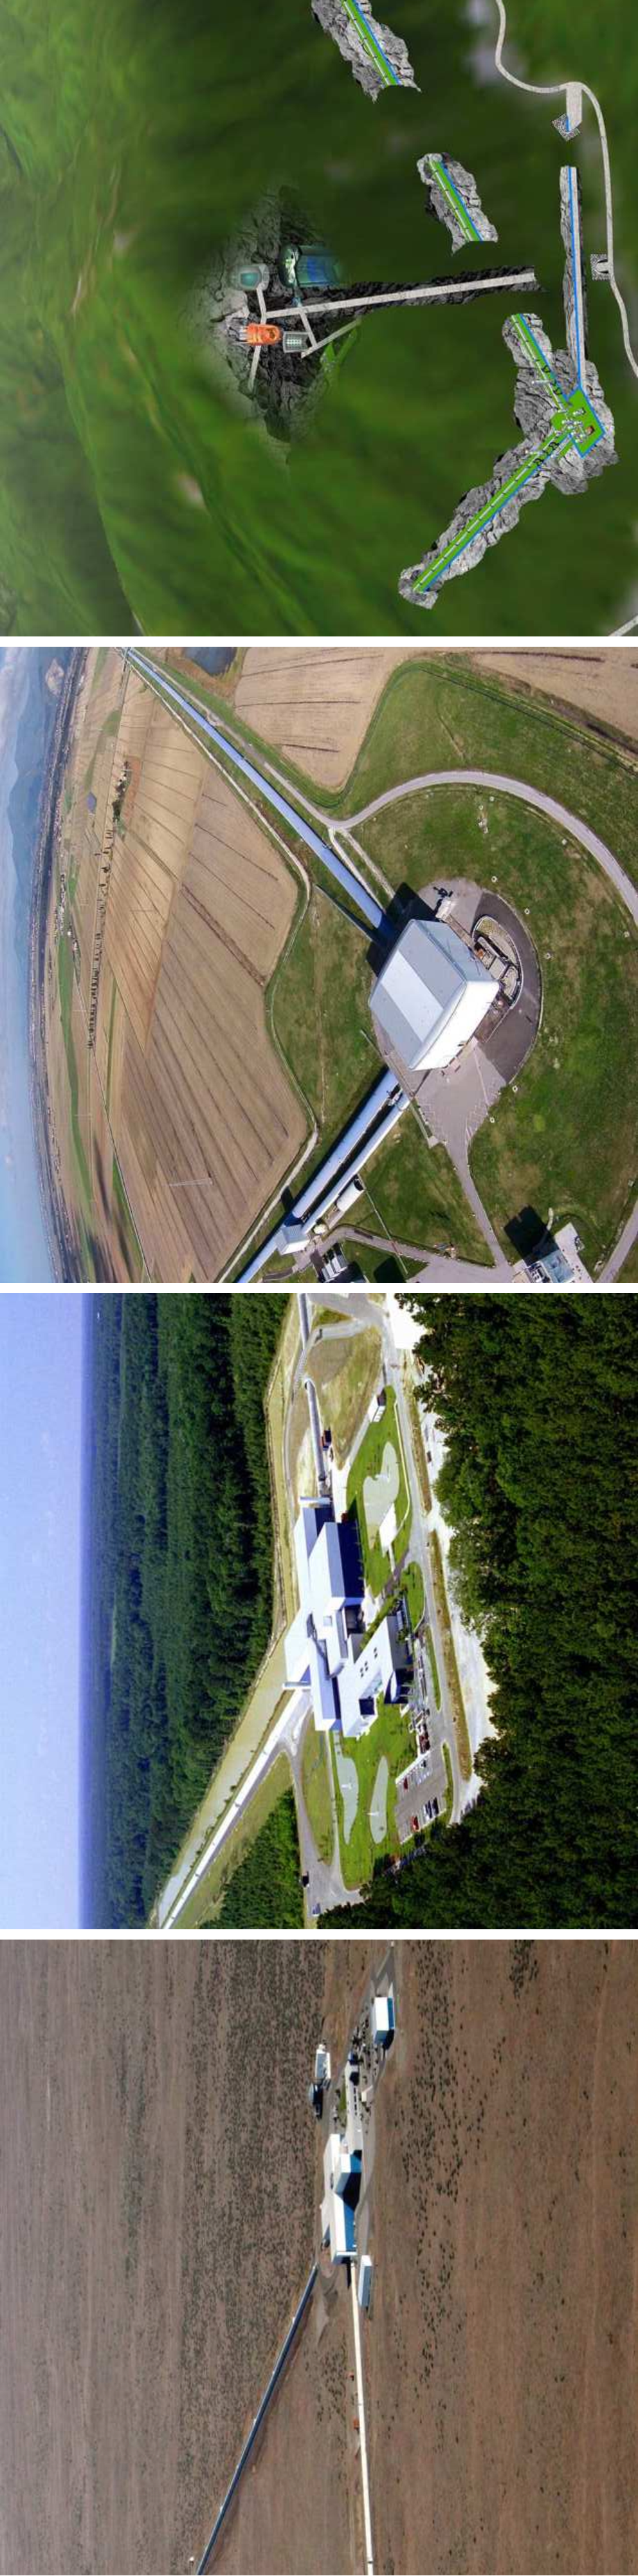
\includegraphics[height=\textwidth,angle=-90]{figures/gwo_ifos-pictures.pdf}
	\end{center}
	\caption{Gravitational wave detectors around the world, in order (left to right): LIGO Hanford, LIGO Livingston, VIRGO, KAGRA. Interferometer arm lengths are on the kilometre scale.}
	\label{fig:gw_ifos}
\end{figure*}

% gw’s and gw detectors
The first direct detection of gravitational waves in 2015 from the merger of two black holes~\cite{GW150914} opened a new frontier for astronomy. 
Gravitational waves are a prediction of the theory of General Relativity and represent ripples in the ``fabric of space-time'' that stretch and squash the lengths and durations between events. Gravitational wave detectors, including the Advanced Laser Interferometer Gravitational-wave Observatory (aLIGO~\cite{AdvancedLIGO:2015}), are vast and complex experiments that rely fundamentally on the interference of light to detect minuscule changes in the lengths of the two long arms of an interferometer, such as those shown in Fig.~\ref{fig:gw_ifos}. Currently, detectable gravitational waves are limited to come from transient, massive cosmic sources, such as the mergers of binary black holes and neutron stars~\cite{GWTC-1:2018}. With the initial generation of detectors having demonstrated that detection is possible, the natural question is how to improve upon them to make detectors with higher sensitivity for all kinds of sources. Possible future sources include higher frequency signals, continuous gravitational waves from rotating neutron stars~\cite{SuvorovaEtAl:2016}, and early universe observations.


% motivate the need for optical modelling
Due to the complexity of the detectors, deriving analytic solutions for the expected signal and noise output due to a passing gravitational wave is difficult to do, and is impossible to do exactly. %, and almost never into a closed form. 
While solutions are known for the current configurations, with each new proposed configuration a new set of non-trivial analytics needs to be done. And as the proposals get more exotic the task only grows more tedious.
One solution is to use optically modelling tools that can deliver fast results and let the researcher quickly ascertain the efficacy of a proposed configuration. 


% what we do
In this report, we demonstrate the use of Finesse~\cite{finesse}, an existing optical modelling software, for a variety of gravitational wave detector configurations and compare against known analytics. In particular, we test the implementation of a non-linear element, a squeezer crystal, in Finesse. We test this component first in a simple cavity and then on proposed detector configurations involving a squeezer inside the signal recycling cavity of the interferometer. This configuration, called ``internal squeezing'', is predicted to improve the quantum noise limited sensitivity around the cavity pole above the currently operational detectors~\cite{Korobko_2019,Adya_2020}. The existing configurations only use a squeezer externally to the interferometer and inject in the squeezed states. By testing this configuration in Finesse we can attempt to verify these claims. 


% report structure
This report is structured as follows.
In Sections~\ref{sec:basics}~\ref{sec:squeezing} we review the basics of interferometry and squeezing, respectively. In Section~\ref{sec:gwIFO} we detail the aLIGO configuration.
In Section~\ref{sec:Finesse} we detail Finesse and what it does.
In Section~\ref{sec:sqzcavity} we test the implementation of a non-linear element in Finesse against derived analytics. %, outside and inside of a cavity.
In Section~\ref{sec:aLIGOcomparison} we compare a model of the aLIGO configuration in Finesse to known analytics, with and without internal squeezing, for a variety of interferometer parameters.
We suggest directions for future work in Section~\ref{sec:future_work} and draw conclusions in Section~\ref{sec:conclusions}.


%%%%%%%%%%%%%%%%%%%%%%%%%%%%%%%%%%%%%%%%%%
\section{Basics of optics for interferometry}
\label{sec:basics}

\subsection{Phase modulation}
% one paragraph
% phase modulation produces sidebands, mirror motion causes phase modulation

The light in a (gravitational wave) interferometer consists of a carrier at around $\omega_0 \approx 10^{14}$ Hz, control and local oscillators at MHz, and noise from classical and quantum sources across the spectrum. Detectable gravitational waves are found with frequencies $\Omega$ between Hz and $10$ kHz. When a gravitational wave passes through the interferometer its effect of stretching or squashing space is akin to the end mirrors in the arms moving back and forth. A moving mirror phase modulates the light incident on it. In the time domain, for a simple sinusoidal carrier $A \cos(\omega_0 t)$ with amplitude $A$ incident on a mirror undergoing small sinusoidal motion at some frequency $\Omega \ll \omega_0$, the reflected light has amplitude $A \cos(\omega_0 t + \delta_m \cos(\Omega t + \phi_m))$ where $\delta_m$ is the modulation depth and $\phi_m$ is the relative phase. To justify the mirror motion being small, given a strain $h(t) \approx 10^{-22}$ from a gravitational wave and an arm length $L \approx 10^3$~m the change in distance is $\Delta L = L h(t) \approx 10^{-19}$ m, far smaller than the radius of a proton ($10^{-15}$ m).


In the frequency domain, taking a Taylor expansion assuming the modulation is weak ($\abs{\delta_m} \ll 1$), the modulation appears as sidebands at $\omega_0 \pm \Omega$, at phase $\pi/2$ ahead of the carrier and amplitude proportional to the modulation depth.
Weak amplitude modulation of the form $A (1 + \delta_m \cos(\Omega t + \phi_m)) \cos(\omega_0 t)$, not considered in depth here, similarly results in faint sidebands at $\omega_0 \pm \Omega$ but in phase with the carrier.


Gravitational waves therefore create weak signal sidebands in the arms of the interferometer. Noise sources (including quantum noise which we consider here) can also shake the mirrors and create their own sidebands of comparable magnitude in the same frequency range. Measuring the signal sidebands despite the noise is the role of the rest of the detector, see Section~\ref{sec:squeezing}.


\subsection{Types of optical cavities}
% one paragraph
% interference of reflected field and circulating field
% Coupled, overcoupled, undercoupled

In gravitational wave detectors many cavities are used to perform a variety of functions, see Section~\ref{sec:gwIFO}. Any cavity is equivalent to a two mirror cavity. Consider two lossless mirrors with reflectivities $r_1$ and $r_2$ separated by a space of macroscopic length $L$. Meaning that it is tuned to the wavelength $\lambda$ of the light and is actually of length $\lfloor \frac{L}{\lambda} \rfloor \lambda$. Of the light incident on mirror 1 from outside the cavity, $\abs{r_1}^2$ of the power is reflected directly off and undergoes no phase change (using the convention of no phase change on reflection and $\pi/2$ on transmission). The light that enters the cavity will either continue to circulate or eventually leave through either mirror. The circulating light that eventually leaks back out through mirror 1 has undergone a phase change of $\pi$ and so will destructively interfere with the directly reflected light. The result of this is that the power ratio of the incident to the reflected light, by working in the frequency domain, is given by~\cite{Danilishin_2012}
$$\abs{\frac{E_{\mathrm{refl}}}{E_{\mathrm{inci}}}}^2 = \abs{\frac{r_1 - r_2 e^{-i 2 L \frac{2\pi}{\lambda}}}{1- r_1 r_2 e^{-i 2 L \frac{2\pi}{\lambda}}}}^2.$$ 

The result of which is that Fabry-Peroy cavities (the ones we’re studying here) fall into three categories determined by which of the two reflected fields dominate, which depends on the relative size of $r_1$ and $r_2$. If $r_1 = r_2$ then the cavity is impedance matched, the fields exactly balance and no light is reflected back. If $r_1 < r_2$ then the cavity is overcoupled, the transmitted circulating fields wins out and light is reflected off the cavity at a $\pi$ phase shift. And if $r_1 > r_2$ then the cavity is undercoupled, the directly reflected field wins out and the light is reflected back at the same phase it came in at. In gravitational wave detectors both overcoupled cavities (e.g.\ the arm cavities) and impedance matched cavities (e.g.\ the power recycling cavity, when no reflection is necessary) are used.


If the reflectivies are fixed and instead the frequency of the incoming light is changed, then resonance peaks are seen in the power of the circulating field whenever the roundtrip distance is some multiple of the wavelength. The distance between these peaks, the free spectral range (FSR), is therefore given by $$\mathrm{FSR} = \frac{c}{2L}.$$ Comparing this to the full-width at half-max (FWHM) of each peak gives a dimensionless rating for the cavity that allows for different cavities to be compared, the finesse (cf.\ the quality factor of an oscillator) $$\mathrm{finesse} = \frac{\mathrm{FSR}}{\mathrm{FWHM}}.$$ For reference, the aLIGO arm cavities have a finesse of $440$~\cite{AdvancedLIGO:2015}.


\section{Generation and detection of squeezed states}
\label{sec:squeezing}

\subsection{Squeezed states}
% one paragraph

Given a sinusoidal signal, one can decompose it into two quadratures $A_C \cos(\Omega t) + A_S \sin(\Omega t)$, called the cosine and sine or the amplitude and phase quadratures (so called because of the effects of amplitude and phase modulation being seen in their respective quadratures). Note that the quadrature decomposition of all the light in the interferometer is relative and taken (typically) with respect to the carrier.


We are interested in quadratures because they lead to a simple explanation of squeezing. In the quantum mechanical two-photon formalism~\cite{Danilishin_2012}, the quadratures relate the harmonic oscillator creation/annihilation operators of the sidebands ($\hat{a}_{\omega_0 \pm \Omega}^\dagger, \hat{a}_{\omega_0 \pm \Omega}$) around the carrier. Assuming that $\Omega \ll \omega_0$, these are related by
\begin{align*}
\hat{a}_c(\Omega) &\approx \frac{1}{2^{1/2}} (\hat{a}_{\omega_0 + \Omega} + \hat{a}_{\omega_0 - \Omega}^\dagger),\\
\hat{a}_s(\Omega) &\approx \frac{1}{i 2^{1/2}} (\hat{a}_{\omega_0 + \Omega} - \hat{a}_{\omega_0 - \Omega}^\dagger).
\end{align*}
In quantum optics, these then define dimensionless “position” and “momentum” operators $\hat{X}, \hat{Y}$, the moments of which describe the uncertainty in each quadrature (and are also equal to values in the spectral density and covariance matrices~\cite{Danilishin_2012}). These uncertainties are equivalent to uncertainty in the amplitude and phase of the electric field.


Consider a vacuum state, although the expected value for either quadrature is zero $\langle \hat{X} \rangle = \langle \hat{Y} \rangle = 0$, due to the Heisenberg Uncertainty Principle (HUP) the standard deviations are limited by $\mathrm{Var}[\hat{X}]^{1/2} \mathrm{Var}[\hat{Y}]^{1/2} \geq 1/2$. Imagining the distribution of the state in $X \times Y$ phase space, this means that smallest area the noise ellipse corresponding to one standard deviation can have is $1/2$. The vacuum ground state with minimum uncertainty has equal radii of $1/2^{1/2}$.


Squeezing a state simply scales one quadrature variance down by some factor while scaling the other quadrature variance up by the same factor, as to maintain the HUP. In phase space, this looks like squeezing (hence the name) the circular noise ellipse: one of its radii decrease and the other increases such that the area remains the same. A squeezer requires two parameters, the squeezing strength $r_{\mathrm{dB}} = 20 \log_{10}(e^r)$ and the squeezing angle $\phi_{\mathrm{sqz}}$. The squeezing strength measures, in dB, the gain in the squeezed quadrature. For a squeezed (vacuum) state the radii get scaled to $e^{\pm r}/2^{1/2}$. The squeezing angle determines along which line the noise ellipse is squeezed.

\subsubsection{Spectral density}

% spectral density of the quantum noise
The goal of squeezing in a gravitational wave interferometer is primarily to control the quantum noise in a given quadrature. By squeezing the vacuum input (see Section~\ref{sec:gwIFO}) we change the spectrum of the quantum noise, reducing the noise in one quadrature while worsening it in the other. The (double-sided) power spectral density (PSD) $\hat{S}_Z$ of the quantum noise $\hat{Z}$, given a spectrum $\hat{Z}(\Omega)$, is given by $$\hat{S}_Z(\Omega) 2 \pi \delta(\Omega - \Omega') = \langle0| \hat{Z}(\Omega) \circ \hat{Z}^\dagger(\Omega') |0\rangle$$ where $|0\rangle$ is the vacuum state and $\circ$ is the symmetric product $A \circ B = \frac{1}{2}(A B + B A)$. However, the convention for measuring sensitivity (cf.\ power versus amplitude quantities) means that values are reported in dB defined as $20 \log_{10}(I(\Omega)/I(0))$ for a spectrum (typically of intensity, or the power off the photodiode) $I(\Omega)$.
% Throughout, these arguments $\Omega$ are sideband frequencies relative to the carrier.


\subsection{Generation of squeezed states}

In the lab, squeezed states are generated in a non-linear crystal in which parametric down conversion (PDC) occurs stimulated by a pump laser. In degenerate squeezing, a photon of pump frequency $2\omega_0$ is annihilated and two photons of frequency $\omega_0$ are created (called the signal and the idler). The non-linear crystal is directional in that squeezing of light only occurs if the light passes one direction through the crystal, in the other direction the light is unaffected.


In the analytics used here, squeezing is performed by suitable multiplication of the quadrature amplitudes by a squeezing matrix. Given a squeezer parameter $r$ as input, the squeezing strength (or, the amount of signal gain) in dB is given by $r_{\mathrm{dB}} = 20 \log_{10}(e^r)$. The analytics also accounts for the directionality of the squeezer crystal.


In the non-linear element (NLE) implementation in Finesse, squeezing is performed by similar quadrature manipulation as the analytics. However, given a gain value in dB as input, the NLE will produce twice that amount of squeezing as output. In other words, the NLE treats the dB input as $10 \log_{10} (e^r)$ (a power quantity) instead of the conventional $20 \log_{10} (e^r)$ (an amplitude quantity). This can be seen in Fig.~\ref{fig:testing_Finesse_squeezers}, the right panel displays the NLE while the left panel displays the other squeezer component, “sq”, which behaves conventionally. Additionally, the NLE will squeeze states incident from either side, it is direction-less. These differences will be apparent in the results shown, see Sections~\ref{sec:sqzcavity}~\ref{sec:aLIGOcomparison}.

\begin{figure*}%
    \centering
    \subfloat[\centering ]{{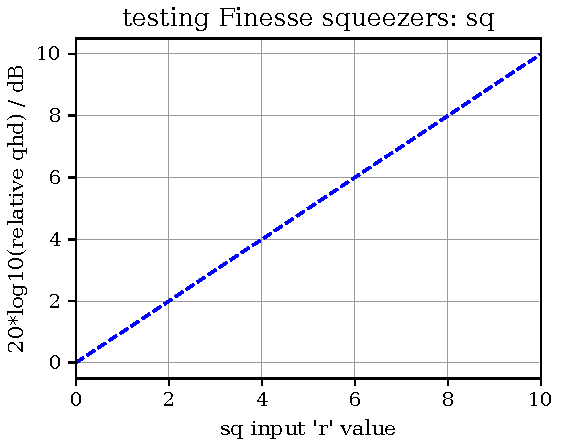
\includegraphics[width=0.4\textwidth]{figures/testing_Finesse_squeezers-sq.pdf}}}%
    \qquad
    \subfloat[\centering ]{{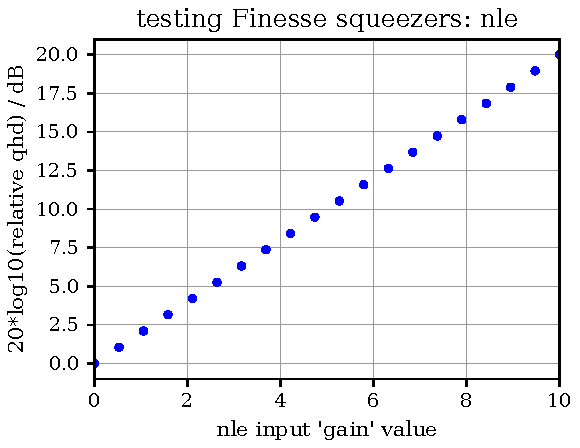
\includegraphics[width=0.415\textwidth]{figures/testing_Finesse_squeezers-nle.pdf}}}%
    \caption{Squeezers implemented in Finesse, showing dB gain (as $20 \log_{10}$) versus input parameter}%
    \label{fig:testing_Finesse_squeezers}%
\end{figure*}

\subsection{Homodyne readout}
% one paragraph

To detect the faint signal sidebands we use a readout scheme. In homodyne readout, the signal is mixed with a strong local oscillator at a beamsplitter. The local oscillator comes from a second laser at the carrier frequency $\omega_0$ but with some relative phase to the carrier, called the homodyne angle $\phi_{\mathrm{LO}}$. After the beamsplitter, the two mixed beams, with different relative phases between the signal and local oscillator, are each read by a photodiode. The output currents are then subtracted (e.g.\ at an op~amp) to obtain the homodyne current, proportional to the difference in intensities at the photodiodes. Homodyne readout in a simplified aLIGO configuration is shown inside the dashed blue box in Fig.~\ref{fig:aLIGO_configuration}.


The resulting homodyne current is proportional to the amplitude of the local oscillator times a combination of the sideband quadrature amplitudes dependent on $\phi_{\mathrm{LO}}$, yet is independent of any laser noise from the local oscillator. Appropriate choice of $\phi_{\mathrm{LO}}$ allows the squeezed quadrature to be extracted. Note that homodyne readout does nothing to reduce the noise in the sidebands, it just allows for the benefits of squeezing to be gained by filtering out the anti-squeezed (or worsened) quadrature.


%%%%%%%%%%%%%%%%%%%%%%%%%%%%%%%%%%%%%%%%%%
\section{Gravitational wave detector interferometry}
\label{sec:gwIFO}

\subsection{The Michelson interferometer}
% one paragraph

\begin{figure*}
	\begin{center}
	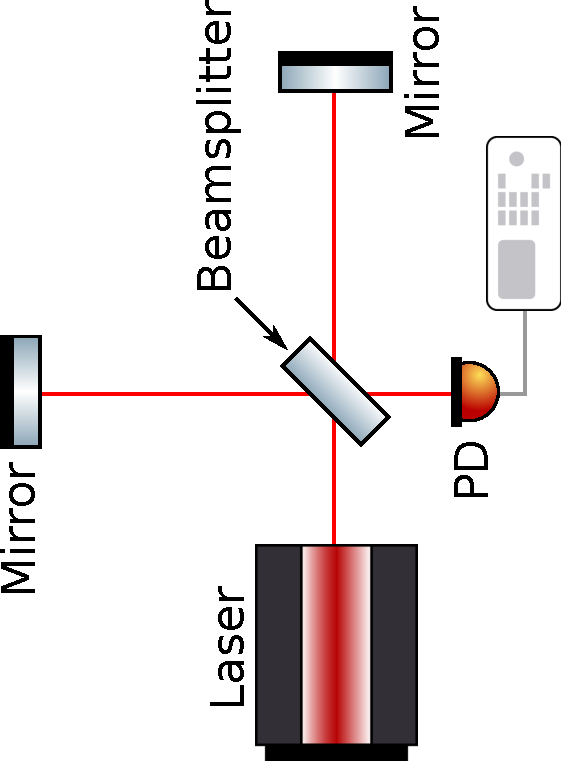
\includegraphics[height=0.5\textwidth,angle=-90]{figures/Michelson_interferometer.pdf}
	\end{center}
	\caption{Configuration of a simple Michelson interferometer}
	\label{fig:Michelson}
\end{figure*}

In its simplest form (ignoring spatial effects henceforth), a Michelson interferometer consists of a laser, a beamsplitter, two arm mirrors, and a photodiode. The laser light is split and travels down two arms, reflects of a mirror at the end of each arm, and then recombines at the beamsplitter output, at which a photodiode is placed. The relative path difference between the two arms produces interference at the photodiode. By tuning the unperturbed lengths of the arms the photodiode can default to being the darkport of the interferometer (or in practise, slightly off the darkport). As such, if something perturbs the arms (e.g.\ noise or a gravitational wave) in a manner to change the relative path difference, then the photodiode will measure some light.


\subsection{Configuration of aLIGO}
% (not investigated here): external squeezing, mode cleaning and spatial effects

\begin{figure*}
	\begin{center}
	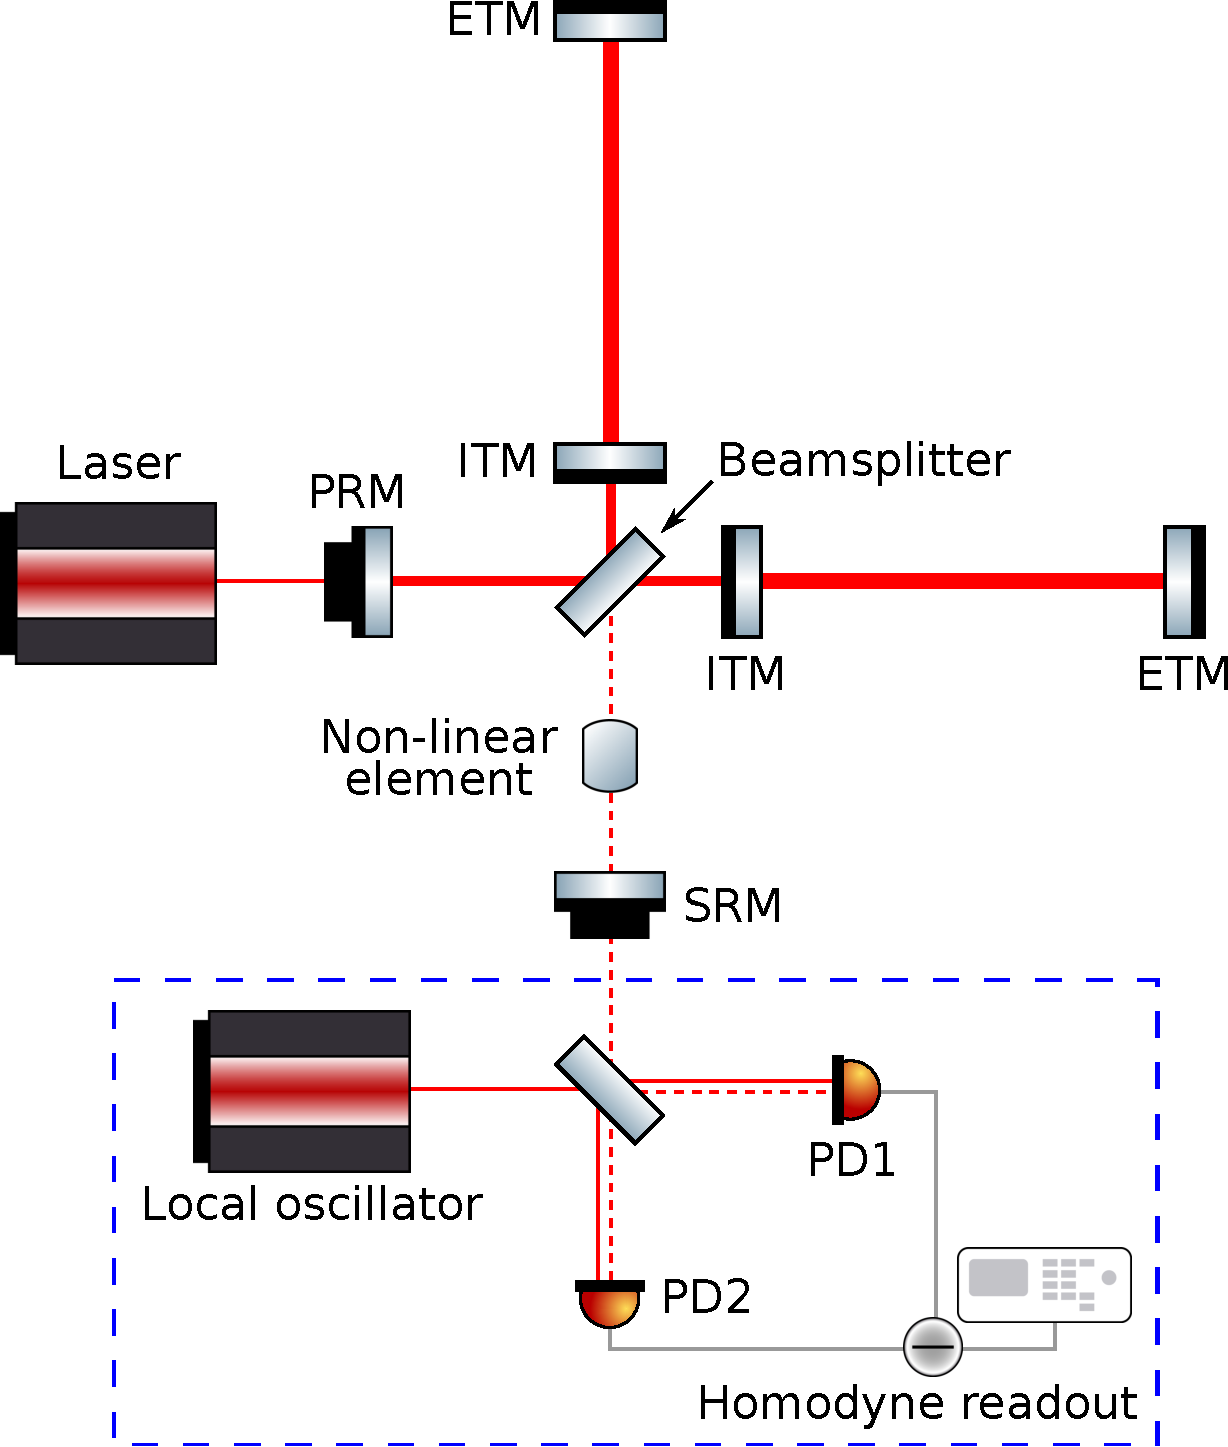
\includegraphics[width=0.7\textwidth]{figures/aLIGO_internal_squeezing.pdf}
	\end{center}
	\caption{Simplified configuration of aLIGO}
	\label{fig:aLIGO_configuration}
\end{figure*}
We study a simplified aLIGO configuration, shown in Fig.~\ref{fig:aLIGO_configuration}, and provide motivation for each component.


In the farfield, a gravitational wave stretches and squashes the distances between objects in a quadrupole manner. Transverse to the axis of propagation distances in one direction are stretched while those in the perpendicular direction are squashed. In order to best detect these changes we need two pairs of objects at right angles to each other (and, ideally, to the gravitational wave). For this we introduce another mirror into each of the beam arms, forming an overcoupled arm cavity between an initial test mass (ITM) and an end test mass (ETM).


% arm cavities, prc, src, 
To achieve the sensitivity required for gravitational wave detection, a classical Michelson interferometer requires technically infeasible amounts of power in the arms in order to reduce the shot noise, see Section~\ref{sec:noise_sources}.
To achieve high power in the arms, a power recycling mirror (PRM) is introduced before the beamsplitter, this reflects power returning from the arm cavities back into the interferometer. For reference, in aLIGO a $125$ W laser results in $\approx 5$ kW of power incident on the beam splitter and beyond $600$ kW of power in the arms.


For a passing gravitational wave to result in detectable changes in the arm lengths, the beam arms need to be at least kilometres long (e.g.\ $4$ km long in aLIGO). To increase sensitivity, the signal from the darkport of the beamsplitter can be amplified by reflecting it back into the arms to ``see'' the gravitational wave again. This is done by placing a signal recycling mirror (SRM) after the darkport of the beamsplitter. What the signal recycling cavity (SRC) actually does is more complicated, see Section~\ref{sec:long_srcs}.


\subsubsection{Reduction of aLIGO to coupled cavities}
% simplification to coupled cavities

\begin{figure*}
	\begin{center}
	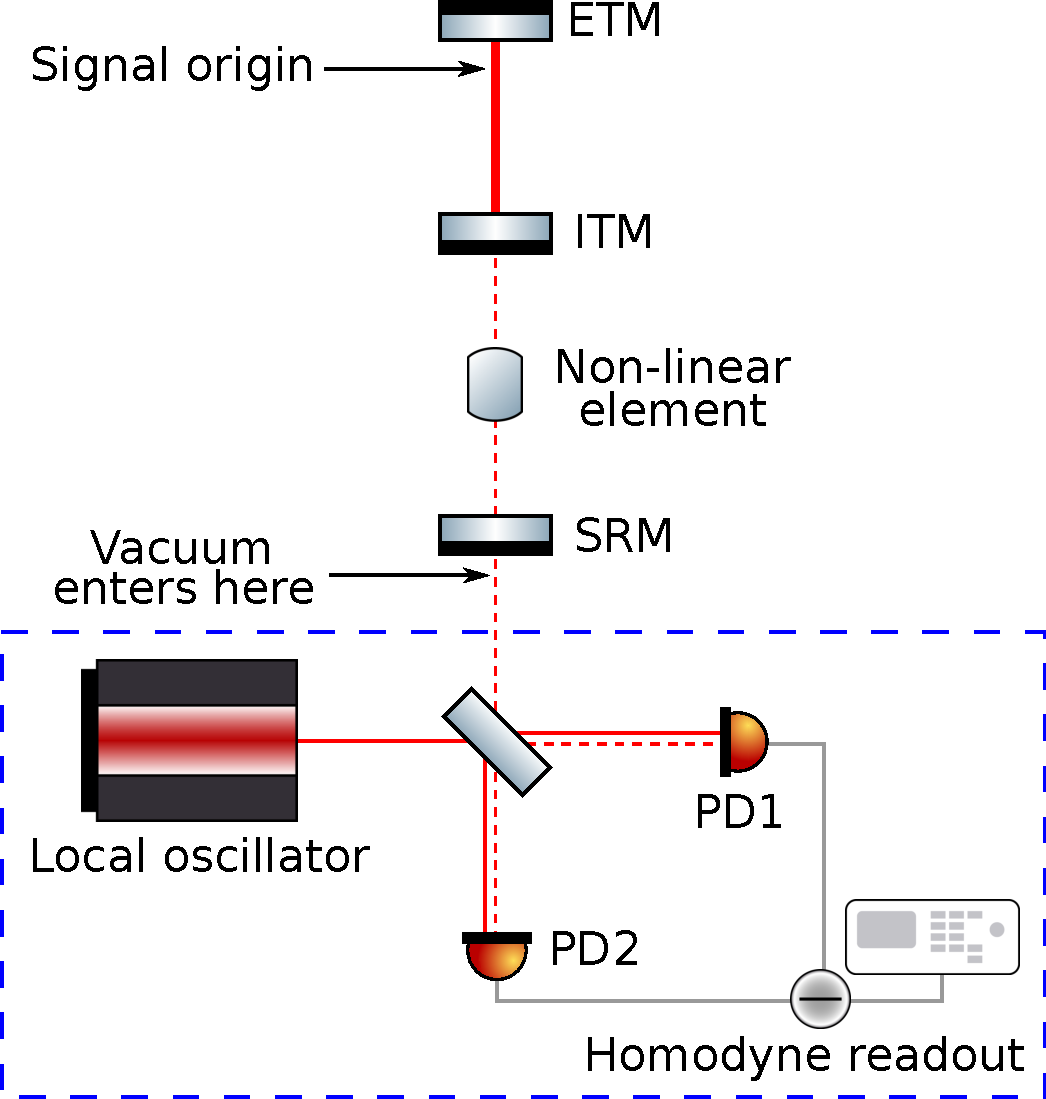
\includegraphics[width=0.7\textwidth]{figures/aLIGO_as_coupled_cavities.pdf}
	\end{center}
	\caption{Reduced configuration of aLIGO to coupled cavities}
	\label{fig:aLIGO_as_coupled_cavities}
\end{figure*}

Despite all the components in the (simplified) aLIGO, the resultant transfer functions for the signal and the noise are equivalent (to a good approximation) to those for two coupled cavities, shown in Fig.~\ref{fig:aLIGO_as_coupled_cavities}. The differential mode from the two arms becomes an optomechanical coupling between the SRC and the beam arm.
Although the coupled cavity system isn’t physical, for example the source of the laser in arm cavity is non-existent, the reduction is useful to understanding the interferometer. In particular, it is clear in the reduced system that the signal and the noise see the cavities differently as they they enter from different sides. This explains how internal squeezing can affect them differently, as discussed in Section~\ref{sec:internal_squeezing}.


\subsection{Noise sources}
\label{sec:noise_sources}
% strain plot, quantum noise limited strain sensitivity
% quantum, Newtonian (seismic), thermal,

\begin{figure*}
	\begin{center}
	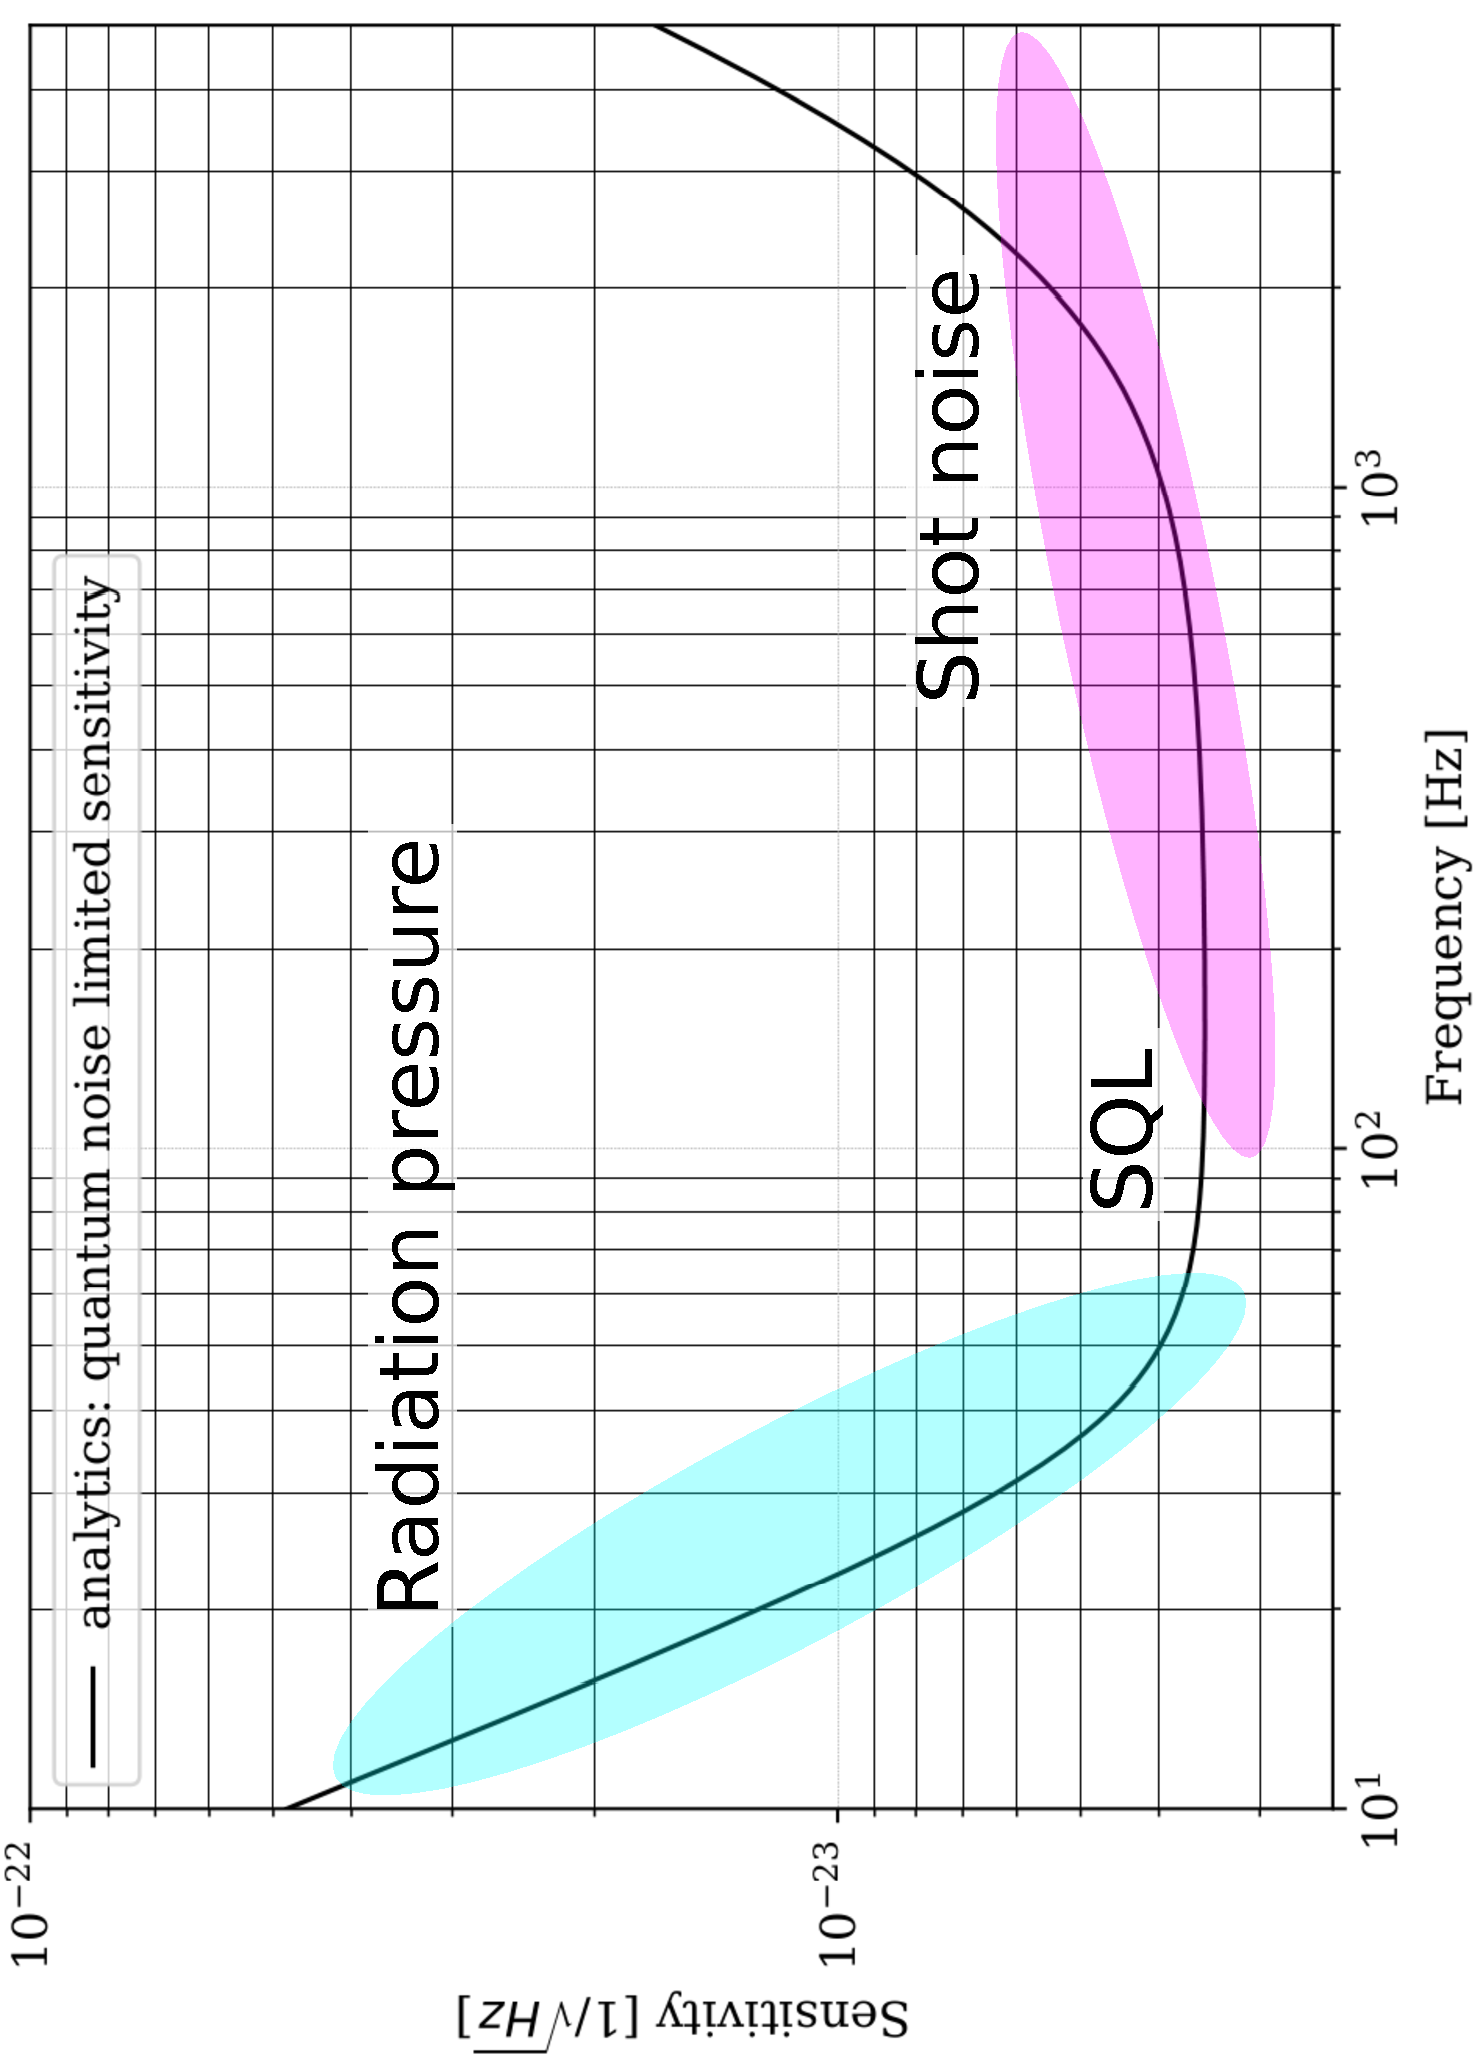
\includegraphics[height=0.8\textwidth, angle=-90]{figures/sqz_aLIGO_analytics_quantum_noise_budget-labelled.pdf}
	\end{center}
	\caption{Quantum noise limited sensitivity of aLIGO (without squeezing), from analytics. Showing the regions where the radiation pressure (blue) or the shot noise (pink) dominate, along with the standard quantum limit (SQL) where they balance.}
	\label{fig:sqz_aLIGO_analytics_quantum_noise_budget}
\end{figure*}


In aLIGO, noise enters the system from many sources and reduces sensitivity across the frequency range of Hz to kHz. Classically, these range from vibrations in the ground (seismic noise) and changing in the nearby distribution of matter (Newtonian noise), to thermal vibration of the components and the space they hang in (thermal noise). Control systems and the natural resonances of the mirror suspensions also remove the possibility for detection in certain bands. We don’t consider these effects here, instead focusing on the quantum noise. We assume that all these noise sources are static in frequency, an often reasonable assumption. 


Quantum noise comes from the fundamental HUP limits on the uncertainty in each quadrature, discussed in Section~\ref{sec:squeezing}. Vacuum enters the interferometer at every open port, most importantly from behind the SRM, and, due to the Fluctuation Dissipation Theorem~\cite{Danilishin_2012}, at every lossy optical component in the form of new, un-correlated noise. In the phase quadrature, quantum noise manifests as shot noise, uncertainty in the number of photons hitting one of the mirrors, that is strongest at high frequencies. In the amplitude quadrature, quantum noise comes as radiation pressure, driving of mirror oscillations by incident light, that is strongest at low frequencies. Increasing the power in the arms reduces shot noise but increases radiation pressure, leading to a trade-off in how much power is put into the interferometer.


To compare noise sources, we define the noise limited strain sensitivity to be the signal amplitude required to achieve a signal-to-noise (SNR) ratio of one, with respect to the given noise source in isolation. This means computing the signal and noise transfer functions for the interferometer and suitably dividing them. The total sensitivity of the interferometer is then then sum of the contribution from each noise source.
In frequency, the maximum sensitivity is achieved for quantum noise where the radiation pressure and shot noise balance, known as the standard quantum limit (SQL), shown in Fig.~\ref{fig:sqz_aLIGO_analytics_quantum_noise_budget}.	


\subsection{Short versus long signal recycling cavities}
\label{sec:long_srcs}

\begin{figure*}
	\begin{center}
	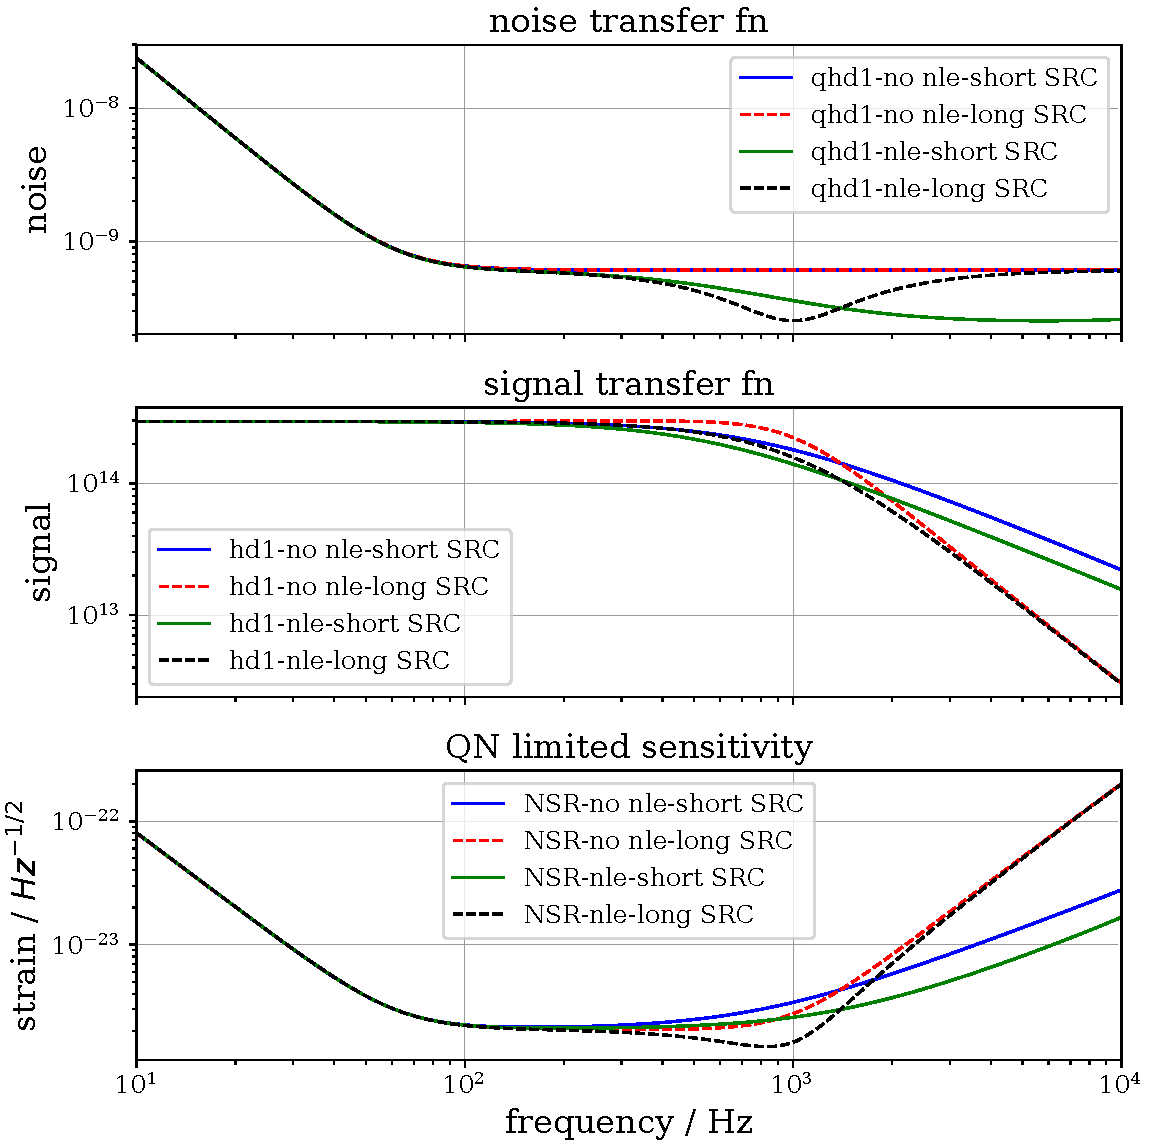
\includegraphics[width=0.9\textwidth]{figures/aLIGO_transfer_fns_and_sensitivity_comparison.pdf}
	\end{center}
	\caption{Signal and noise transfer functions and sensitivity plot for aLIGO configuration modelled in Finesse}
	\label{fig:src_transfer_functions}
\end{figure*}

The signal recycling cavity (SRC) amplifies the signal by reflecting it back into the interferometer, as described above.
% Introduction of the SRC also broadens the FHWM of the cavity reasonance.
Considering the coupled cavity system in analogy to a system of two coupled harmonic oscillators, changing the length of the SRC affects the coupling between the cavities, or the energy transfer between the oscillators. The lowest resonance of the coupled system, known as the coupled cavity pole, changes depth and bandwidth depending on the length of the SRC.


The effect of the length of the SRC on the signal transfer function is shown as red and blue lines in the middle panel of Fig.~\ref{fig:src_transfer_functions}.
For a short SRC, the signal transfer function is constant at frequencies below $10^2$ Hz and then slowly begins to roll off, losing an order of magnitude when it gets to $10$ kHz. For a long SRC (of comparable length to the arm cavity), the signal transfer function is similar at lower frequencies, begins to roll off later than the short SRC, but has a faster roll off thereafter, losing two orders of magnitude by $10$ kHz. As a result, the long SRC is more sensitive around the coupled cavity pole but has shorter bandwidth overall, see the bottom panel of Fig.~\ref{fig:src_transfer_functions}.


Importantly, the length of the SRC also affects how internal squeezing reduces the quantum noise, discussed below.

\subsection{Internal squeezing}
\label{sec:internal_squeezing}

Internal squeezing is when the squeezer crystal is placed inside the interferometer, in the SRC as in Figs.~\ref{fig:aLIGO_configuration}~\ref{fig:aLIGO_as_coupled_cavities}, as opposed to having the vacuum squeezed externally and injected in via an isolator (external squeezing). Note that aLIGO currently uses external and not internal squeezing. Since external squeezing is compatible with internal squeezing~\cite{Adya_2020,Korobko_2019}, it can be included with or without internal squeezing, making it an additional complexity unnecessary to assess the benefits of the internal squeezer to proposed detector configurations. We do not consider external squeezing further here.


% SRC, signal de-amplification
Here we consider a high frequency (HF) gravitational wave detector, where the internal squeezing is in the phase quadrature. As such, the quantum phase noise gets reduced, in particular, around the coupled cavity pole. The length of the SRC affects the bandwidth of the noise reduction, shown in the black and green lines in the top panel Fig.~\ref{fig:src_transfer_functions}.
Squeezing in phase will anti-squeeze in amplitude, but in Fig.~\ref{fig:src_transfer_functions} the homodyne angle is chosen to select the phase quadrature, which explains why there is no effect at low frequencies where the quantum noise is in the amplitude quadrature. 
However, squeezing in phase results in the signal losing-power around the pole (known as de-amplification), however the reduction in noise is more significant and so the sensitivity overall improves around the pole.
% vacuum input, signal and noise see the interferometer differently
Why internal squeezing affects the noise and the signal differently is best understood through the couple cavity system. There, the vacuum and the signal enter the system from different ends (the noise enters into the SRC while the signal is generated in the arm cavity) and so will see the squeezer differently.


The goal of the rest of this report is to test the implementation of internal squeezing in Finesse by considering different detector configurations.


%%%%%%%%%%%%%%%%%%%%%%%%%%%%%%%%%%%%%%%%%%
\section{Finesse} %- Optical modelling
\label{sec:Finesse}
% this section can be quite short

% what does finesse do, how does it do it
Finesse~\cite{finesse} (Frequency domain INterfErometer Simulation SoftwarE) is designed for modelling interferometer configurations. For a specified configuration of optical components, at each connecting node it calculates the amplitudes for the carrier, any control signals, the gravitational wave signal sidebands, and the quantum noise sidebands (see Sections~\ref{sec:basics}). By solving the appropriate matrix equations, it does all of this entirely in the frequency domain.
Although not explored here, Finesse also is able to handle the spatial geometry of Gaussian beams, noise coupling from different parts of the interferometer, and imperfections such as misalignment and higher order modes~\cite{Bond_et_al_2016}.
By placing appropriate detectors at the output, Finesse is able to calculate the expected signal and quantum noise transfer functions and so the sensitivity of a proposed detector configuration, which is what we are interested in modelling (see Section~\ref{sec:aLIGOcomparison}) and which has already been done for gravitational wave detector commissioning~\cite{brown2020pykat}.


% what is new
Newly implemented in Finesse is a non-linear element component. Unlike the existing squeezer component, this can be placed anywhere within the configuration. The modelling of this component was based on similar analytics to those in Appendix~\ref{app:squeezed_cavity_analytics}. We are interested in both testing if this component is implemented correctly and in using it to examine proposed detector configurations with internal squeezing. Although, applications of the non-linear element are not limited to gravitational wave detector modelling.


% how we use it
We interact with the simulation through a Python~\cite{python} wrapper called PyKat~\cite{brown2020pykat}, in particular, this allows for optimisation routines and plotting do be done in Python in order to find optimal configurations. All of our working and implementation is documented and available at \url{https://github.com/daccordeon/aliveKat} as open source software.


%%%%%%%%%%%%%%%%%%%%%%%%%%%%%%%%%%%%%%%%%%
\section{Modelling a squeezed cavity} %a non-linear element in a cavity
\label{sec:sqzcavity}

\begin{figure*}
	\begin{center}
	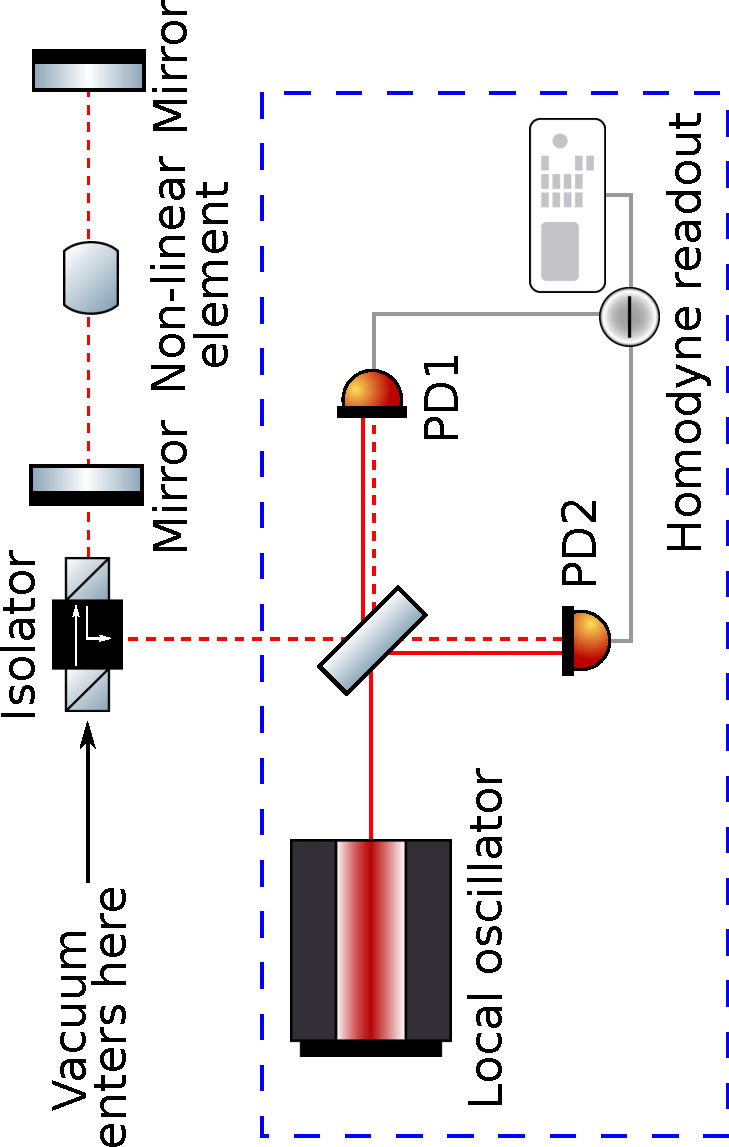
\includegraphics[height=0.7\textwidth, angle=-90]{figures/squeezed_cavity.pdf}
	\end{center}
	\caption{Configuration of squeezed cavity}
	\label{fig:squeezed_cavity}
\end{figure*}

\subsection{Analytics}

% approximate noise sources/vacuum to just come from ...
To first test the non-linear element we consider a simpler system than aLIGO, a squeezed cavity, as shown in Fig.~\ref{fig:squeezed_cavity}. This consists of a squeezer inside of a cavity, and homodyne readout to detect the squeezed vacuum of quantum noise. An isolator is included to redirect the squeezed output. We simplify by assuming that one of the mirrors is fully reflective (therefore the cavity is overcoupled) and that both mirrors are lossless. We assume that the only noise sources are the vacuum input into the cavity and the laser noise in the local oscillator (which will cancel out as usual in homodyne readout).
% leave the actual derivation to an appendix
We derive the analytics for this system, getting an expression for the power spectral density (PSD) of the homodyne intensity, $S_{\mathrm{HomI}}(\Omega)$, in terms of the parameters of cavity (the reflectivity of the first mirror, the length and tuning), the squeezer (gain and squeezer angle), and the local oscillator (amplitude and homodyne angle). See Appendix~\ref{app:squeezed_cavity_analytics} for the full derivation.


\subsubsection{Threshold}
% threshold results, operating above threshold isn’t physically meaningful for the approximations made to reach these analytics

\begin{figure*}
	\begin{center}
	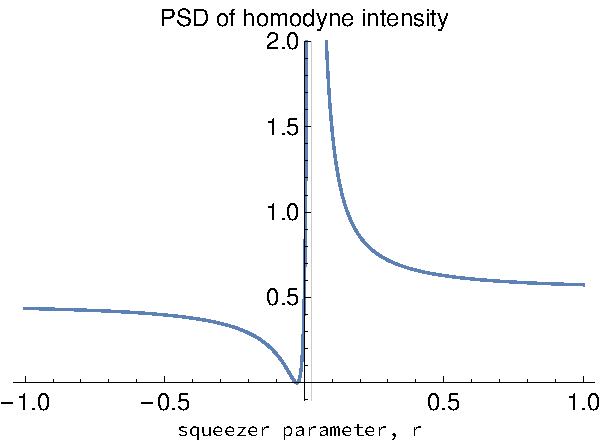
\includegraphics[width=0.6\textwidth]{figures/not_main_PSD_vs_r.pdf}
	\end{center}
	\caption{Analytics result for absolute value of PSD of homodyne intensity against the squeezer parameter for a squeezed cavity}
	\label{fig:not_main_PSD_vs_r}
\end{figure*}

\begin{figure*}
	\begin{center}
	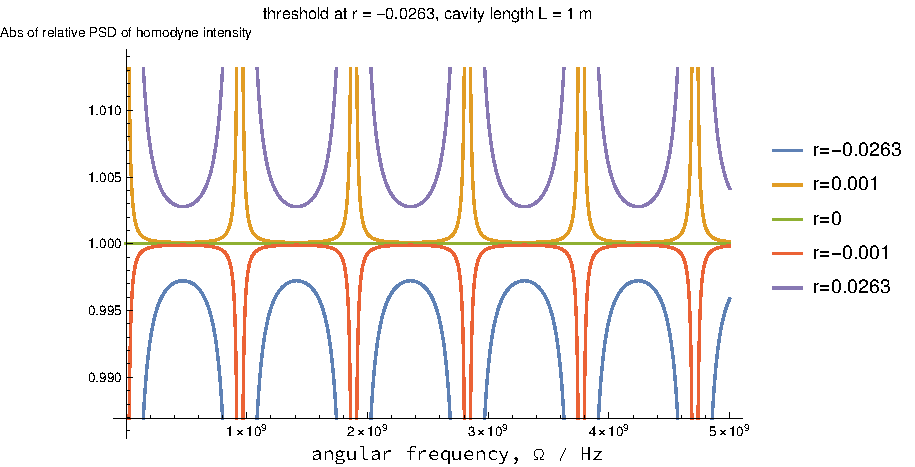
\includegraphics[width=0.8\textwidth]{figures/not_main_PSD_vs_freq.pdf}
	\end{center}
	\caption{Analytics result for absolute value of PSD of relative homodyne intensity against angular frequency offset for a squeezed cavity with various squeezer parameters}
	\label{fig:not_main_PSD_vs_freq}
\end{figure*}

We first consider the behaviour at the carrier frequency of the absolute value of the PSD against the squeezer parameter, i.e.\ $\abs{S_{\mathrm{HomI}}(0)}$ against $r$ (alt.\ $r_\mathrm{sqz}$). We do this for a tuned, $1$ m long cavity, with the first mirror having reflectivity $r_1 = 0.9$, both squeezer and homodyne angle zero (squeezing and readout in the same quadrature), and amplitude $A = 1$ (in suitable units, see derivation), shown in Fig.~\ref{fig:not_main_PSD_vs_r}. This yields a pole at around $r_\mathrm{Thresh} = 0.0263$ (estimated numerically with Mathematica), known as the threshold value for the squeezer. The PSD also has a zero at $r = -r_\mathrm{Thresh}$ and limits to $0.5$ as $\abs{r}$ increases past threshold. Note that the squeezer parameter taking a negative value is equivalent to it taking the absolute value of that value and the squeezer angle changing by $\pi/2$, as in, switching to squeezing in the other quadrature.


The explanation for this behaviour lies in the assumptions made in the analytics. In particular, we assumed that the pump laser for the squeezer, which is its energy source, was essentially an undepletable reservoir. This meant that when we pumped in phase with the noise we could endlessly amplify and we when pumped out of phase we could completely cancel the noise, these two conditions exactly occur when threshold is reached. Physically this is not the case and pump depletion requires a Hamiltonian model of the system to analyse properly. This means that the analytics derived here break at threshold, similarly, any results above threshold are unphysical.
However, the aLIGO squeezer operates normally well below threshold, where the model is reasonably accurate and so can be used to study aLIGO.


We are also interested in the behaviour at some frequency offset $\Omega$ relative to the behaviour at the carrier frequency, i.e.\ $\abs{S_{\mathrm{HomI}}(\Omega)/S_{\mathrm{HomI}}(0)}$ against $\Omega$. For the same parameters as above except for a selection of different squeezer parameters, this is shown in Fig.~\ref{fig:not_main_PSD_vs_freq}. For all non-zero squeezer parameters, it shows resonances every $9.42$ GHz (radians). At each resonance, the threshold values go to infinity and zero, while off resonance they are different from the carrier frequency but remain on the same scale (with difference of order $10^{-3}$).


\subsection{Testing the non-linear element in Finesse}

\begin{figure*}
	\begin{center}
	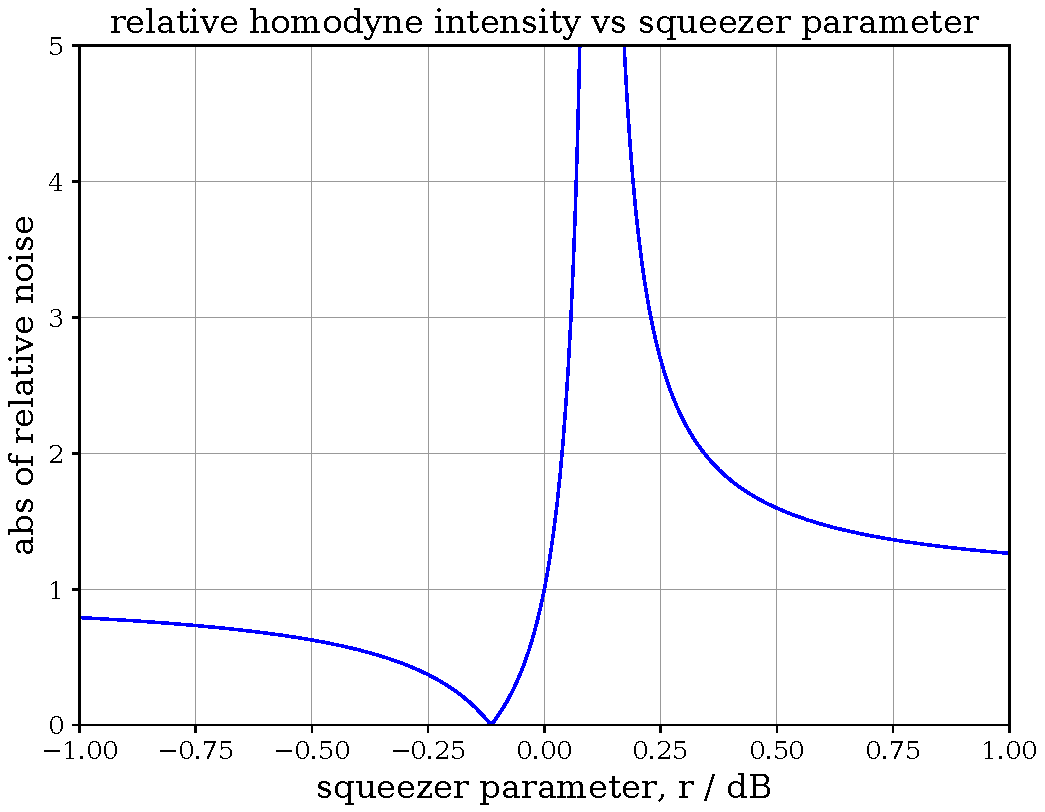
\includegraphics[width=0.7\textwidth]{figures/pykat_relative_qhd_vs_r.pdf}
	\end{center}
	\caption{Finesse result for absolute value of relative PSD of homodyne intensity against the squeezer parameter for a squeezed cavity}
	\label{fig:pykat_relative_qhd_vs_r}
\end{figure*}

\begin{figure*}
	\begin{center}
	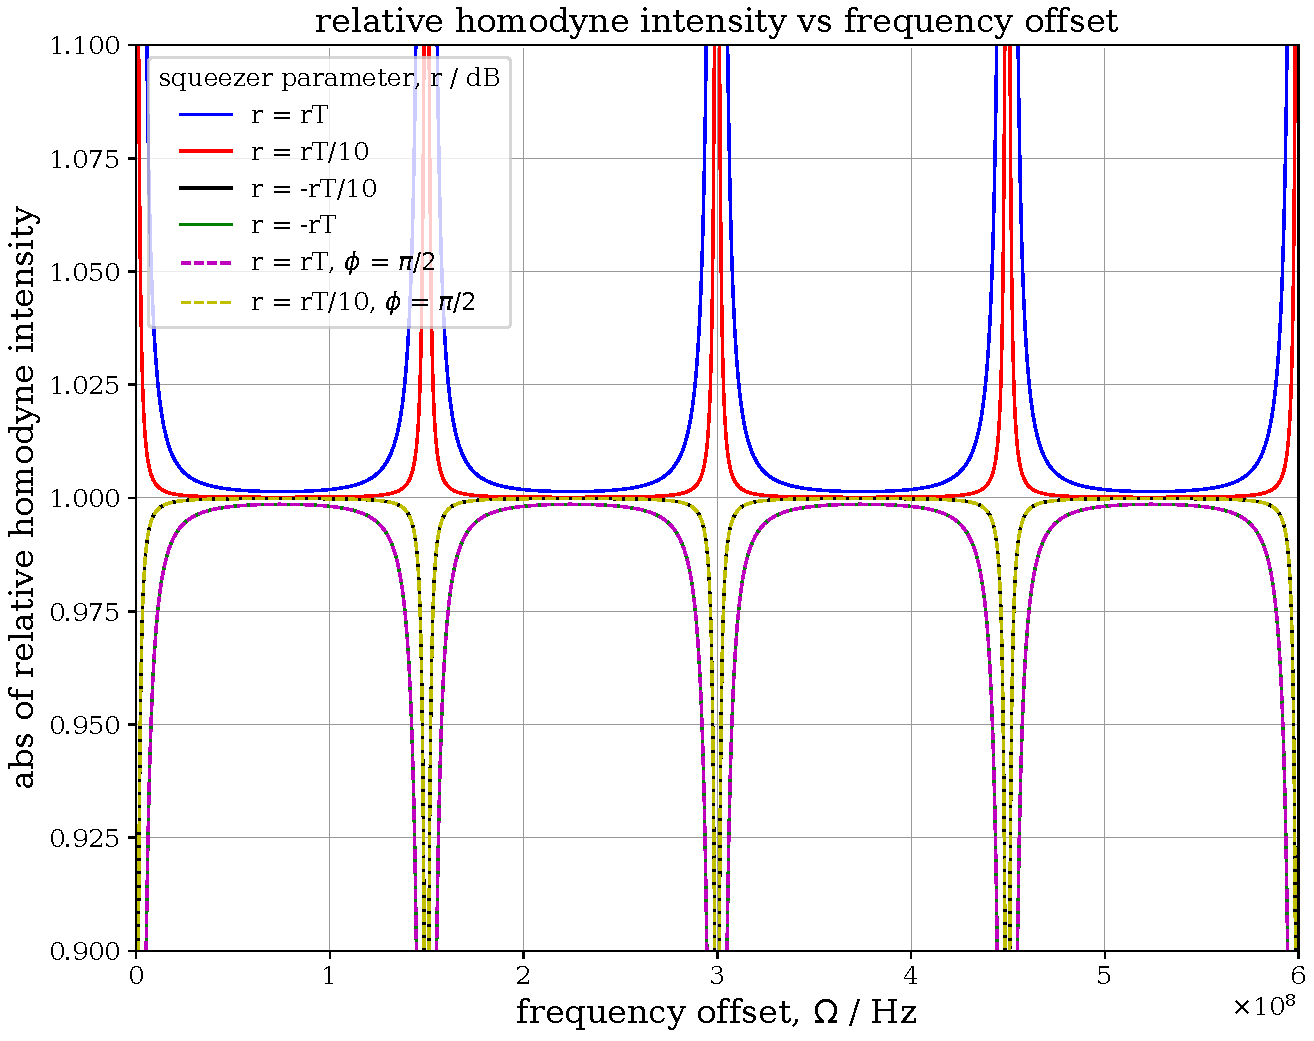
\includegraphics[width=0.8\textwidth]{figures/pykat_relative_qhd_vs_freq.pdf}
	\end{center}
	\caption{Finesse result for absolute value of PSD of relative homodyne intensity against angular frequency offset for a squeezed cavity with various squeezer parameters}
	\label{fig:pykat_relative_qhd_vs_freq}
\end{figure*}

We model the squeezed cavity in Finesse with the \code{nle} component as the squeezer and \code{qhd} for homodyne readout of the quantum noise. We do this for the same parameters as above and only consider the relative spectral density to avoid worrying about units of amplitude. Note that \code{qhd} calculates amplitude spectral density rather than PSD, which under a logarithm gives a factor of two between them, further confusing the definitions of dB.


% rThresh and \Omega values are the same, convert to dB and check angular freq
The behaviour of the relative (spectral density of the) homodyne intensity against the squeezer parameter is shown in Fig.~\ref{fig:pykat_relative_qhd_vs_r}. The shape of the response is similar to the analytics. The squeezer parameter axis shows the input to \code{nle} which is in ``dB'' calculated as $r_{\mathrm{nle}} = 10 \log_{10}(e^{r_\mathrm{sqz}})$. Python quotes the threshold value as $0.144$ (here shown to three s.f.) which agrees with the analytics, $0.114 \approx 10 \log_{10}(e^{0.0263})$, with negligible uncertainty.


% FSR is 1.5 since L = 1
The behaviour against the frequency offset is shown in Fig.~\ref{fig:pykat_relative_qhd_vs_freq}. Again, the response is similar to the analytics. The frequency axis here is actual frequency, rather than the angular frequency shown in the analytics. The FSR here is (up to numerical error) $1.5 10^8$ Hz when $L = 1$ m, which is the predicted $\mathrm{FSR} = c/(2 L) = 3/2 10^8 = 1.5 10^8$ Hz. The FSR in the analytics is $2 \pi$ times this, as expected for the angular frequency. The behaviour against frequency for different squeezer parameters is also similar to the analytics.


Overall, the \code{nle} component successfully models the squeezed cavity, with the consideration for the particular definition of dB used. Now, having passed the first test, we want to test the implementation in a gravitational wave detector to then start predicting the behaviour of proposed designs.


\section{Modelling advanced gravitational wave detector configurations}
\label{sec:aLIGOcomparison}

\subsection{Analytics for the reduced aLIGO configuration}

% get source from Vaishali
We use analytics for the coupled cavity system (shown in Fig.~\ref{fig:aLIGO_as_coupled_cavities}) derived in Refs.~\cite{Korobko_2019,SOMIYA2016521}. Recall that this system is an approximation, albeit a good one, of the simplified aLIGO configuration (shown in Fig.~\ref{fig:aLIGO_configuration}). In addition, the input/output relation and the calculation of the coupled cavity pole are both only approximate. We claim below that these approximations are responsible for the rest of the discrepancy between the analytics and the Finesse model, after first correcting for the implementation in Finesse.


\subsection{Finesse model of aLIGO}

% table of aLIGO parameters used in Finesse model and analytics
\begin{table}
	\centering
	\begin{tabular}{l|ll}
	 & analytics & Finesse \\ \hline
	Arm length / m & 3994.5 & 4000 \\
	SRC length / m & 319 & 319 \\
	Power on beamsplitter / kW & 5.35 & 5.35 \\
	Power in arms / kW & 758.9 & 758.9 \\
	SRM power transmission & 0.12 & 0.12 \\
	ITM power transmission & 0.014 & 0.014 \\
	\textit{Gain input to internal squeezer} & 0.06 & $5 \log_{10}(e^{0.06})$ \\
	Maximum sensitivity / $\mathrm{Hz}^{-0.5}$ & $3.95 \times 10^{-25}$ & $4.16 \times 10^{-25}$ \\
	Peak frequency / kHz & 2.49 & 2.51
	\end{tabular}%
	\caption{Parameters of analytics for reduced and Finesse model for simplified aLIGO configuration with no losses.}
	\label{tab:aLIGO_parameters}
\end{table}

\begin{figure*}
	\begin{center}
	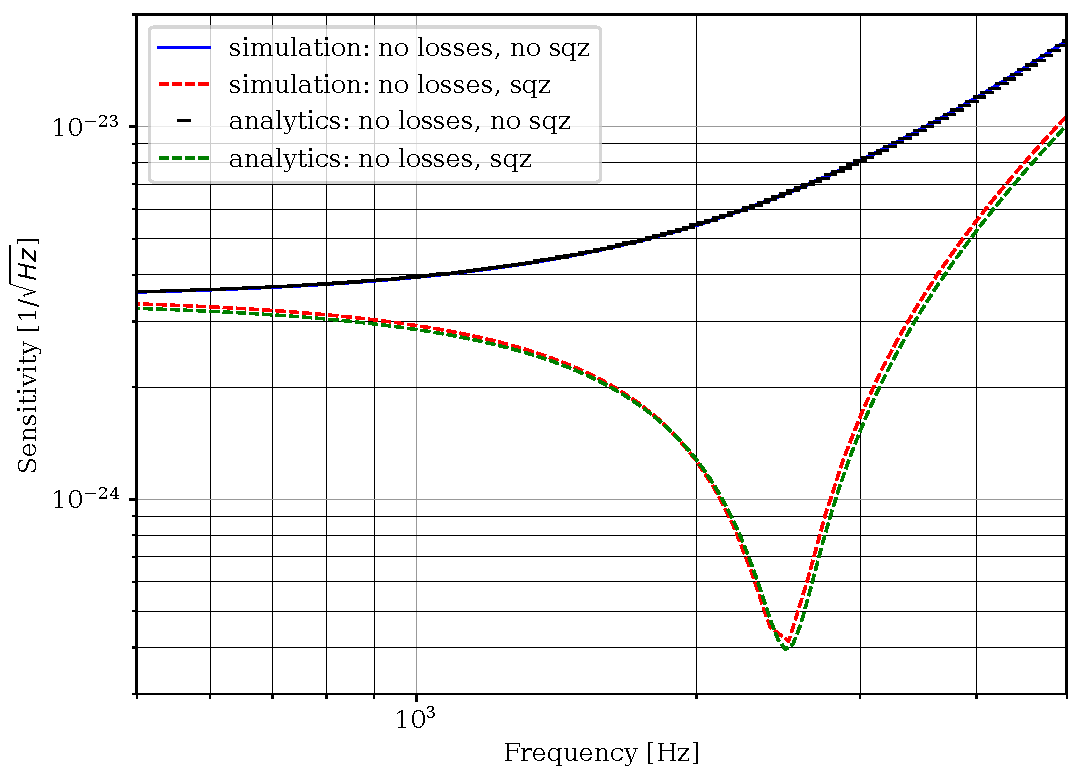
\includegraphics[width=0.8\textwidth]{figures/sqz_aLIGO_analytics_v_simulation.pdf}
	\end{center}
	\caption{Sensitivity of aLIGO for a long SRC with internal squeezing, analytics versus Finesse model.}
	\label{fig:sqz_aLIGO_analytics_v_simulation}
\end{figure*}

We model the simplified, lossless aLIGO configuration (shown in Fig.~\ref{fig:aLIGO_configuration}) in Finesse with internal squeezing using the \code{nle} component. We study a long SRC configuration here, although the agreement between the analytics and model is similar for different parameters. Similar configurations with lengths of the SRC of 53 m and 2 km generate the signal and noise transfer functions and sensitivity shown in Fig.~\ref{fig:src_transfer_functions}. A summary of the parameters used here is shown in Table~\ref{tab:aLIGO_parameters}. Note that the squeezer in the analytics takes the $r_\mathrm{sqz} = 0.06$ parameter as input while the \code{nle} takes the gain in dB (defined as $10 \log_{10}(e^\mathrm{sqz})$ against convention) as input. However, here we input only $5 \log_{10}(e^\mathrm{sqz})$ into the Finesse model, explained below.


% comparison for long SRC with internal squeezing
A comparison of sensitivity of the analytics and Finesse is shown in Fig.~\ref{fig:sqz_aLIGO_analytics_v_simulation}. With the squeezer turned off, the agreement is nearly exact (to numerical error). With the squeezer turned on, the sensitivity is quite similar between the analytics and the Finesse model, with error at the peak sensitivity on the order of $10^{-26}$ and with similar relative error off peak (i.e.\ on a logarithmic scale the error looks uniform across frequency, as seen in Fig.~\ref{fig:sqz_aLIGO_analytics_v_simulation}). This remaining error we attribute to the approximations made in the analytics, in some ways, the Finesse model is more accurate.


\subsubsection{Explaining the discrepancy in dB}

% different def of dB gives a factor of 2
To recap, the squeezer in the analytics takes $r_\mathrm{sqz}$ as input and produces a gain in dB calculated as $20 \log_{10}(e^\mathrm{sqz})$. In Finesse, the \code{nle} components takes a gain value as input but calculates dB as only $10 \log_{10}(e^\mathrm{sqz})$, therefore producing twice the amount of squeezing than expected, as shown in Fig.~\ref{fig:testing_Finesse_squeezers}. This means that given the $r_\mathrm{sqz} = 0.06$ input into the analytics, we need to halve the gain to account for the difference in definitions in dB, and input into \code{nle} $10 \log_{10}(e^\mathrm{sqz})$.


% double passing of NLE gives another factor of 2
However, as seen in Fig.~\ref{fig:sqz_aLIGO_analytics_v_simulation}, the correct value to pass to \code{nle} is $5 \log_{10}(e^\mathrm{sqz})$, so where is the second factor of two? As mentioned in Section~\ref{sec:squeezing}, physical squeezer crystals are directional, meaning that they will only squeeze states incident from one side, letting those incident from the other through unchanged. The implementation of \code{nle} is, however, direction-less, meaning that it squeezes from both sides. When placed in a cavity it produces twice the amount of squeezing than expected. Therefore, given a squeezer parameter (not in dB), the gain in dB to pass to \code{nle} is half as small due to different definitions of dB and half as small again due to the direction-less-ness of the component. This second factor of two was not evident in the squeezed cavity results because there the squeezer in the analytics was directionless.


% Is the recommendation to Daniel Brown to both fix the dB and perhaps make nle a directional component (will squeeze light from n1 to n2, but will just let light through n2 to n1)?
Overall, the \code{nle} component successfully models the simplified aLIGO configuration up some error likely due to approximations in the analytics, with the caveat that the gain input must be corrected to account for the nature of the implementation. This is a good result and resolves, positively, the testing of the \code{nle} component that we set out to do. For the sake of consistency, we recommend that the \code{nle} component be modified to calculate the gain as $20 \log_{10}(e^\mathrm{sqz})$ and possibly made directional.


\subsection{Optimisation}

\begin{figure*}
	\begin{center}
	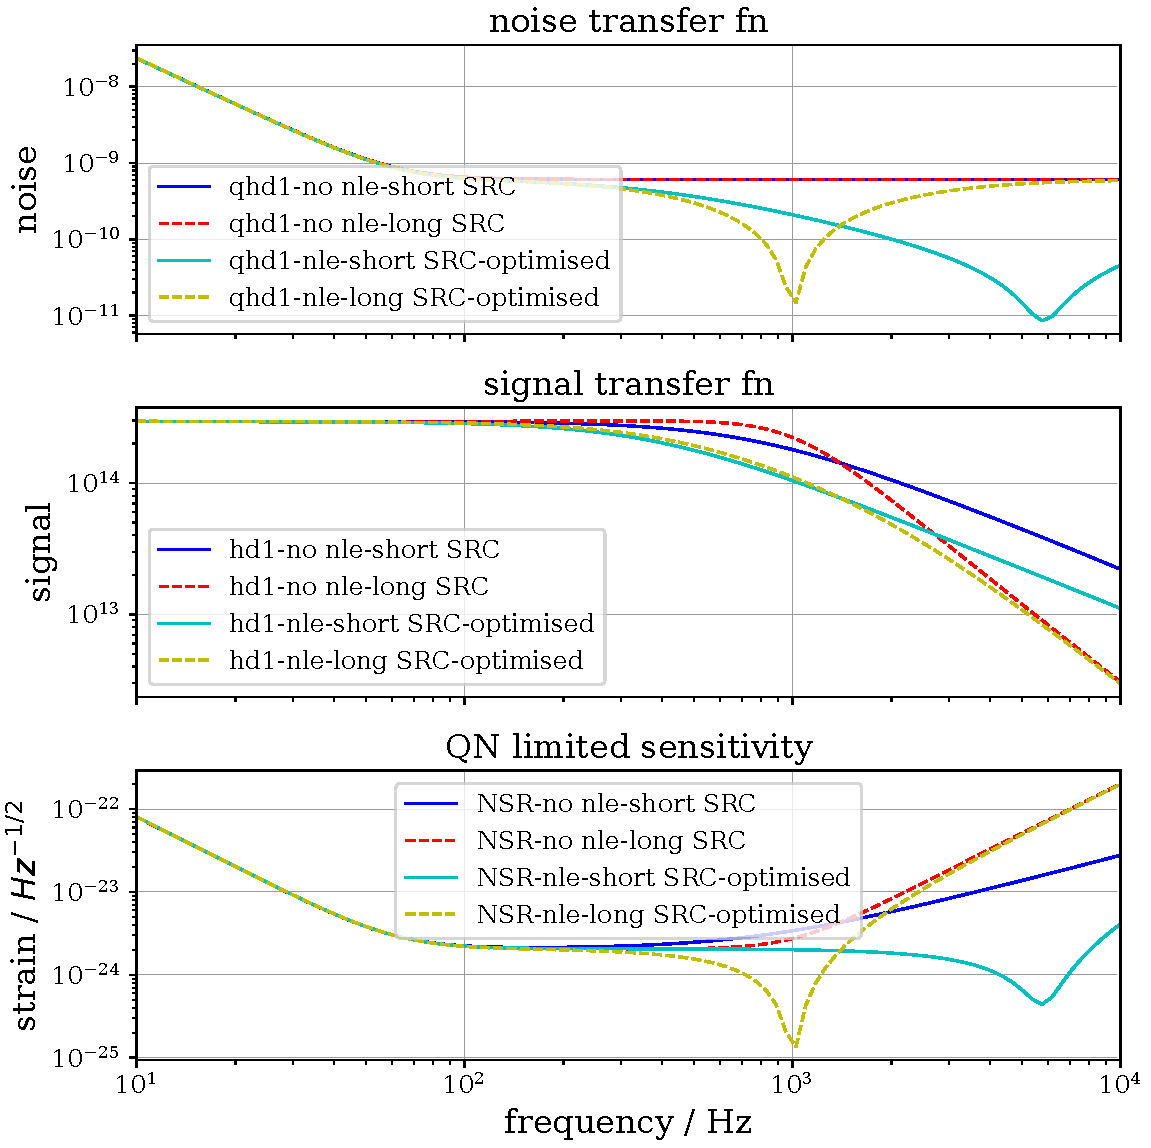
\includegraphics[width=0.8\textwidth]{figures/aLIGO_optimum_sensitivity_comparison.pdf}
	\end{center}
	\caption{Optimised sensitivity for fixed lengths of the SRC, for Finesse model of aLIGO with internal squeezing.}
	\label{fig:aLIGO_optimum_sensitivity_comparison}
\end{figure*}

% reason to use python is to optimise
Having successfully shown that Finesse can model the aLIGO configuration, we can now use PyKat to optimise the sensitivity in some band against whatever parameters we like. Here we only do this briefly, as a demonstration of the ability, but more broadly this is a key benefit of Finesse.


We optimise the sensitivity within a high frequency band of 900 Hz to 3 kHz for fixed lengths of SRC of 53 m and 2 km, the results are shown in Fig.~\ref{fig:aLIGO_optimum_sensitivity_comparison}. The optimisation was allowed to vary the squeezer gain, the squeezer angle, and the homodyne angle. Once again the results show the high peak, short bandwidth of the long SRC which achieves a sensitivity of $1.36 \times 10^{-25}\; \mathrm{Hz}^{-0.5}$. It achieves this at a non-zero squeezer angle of $0.014^\circ$, which is surprising and not yet understood (although it could just be the optimisation routine). Allowing the optimisation to vary additionally the length of the SRC, the power transmission of the SRM, and the tuning of the SRM led to the optimisation getting stuck near the various initial values given, for reasons not yet understood.


%%%%%%%%%%%%%%%%%%%%%%%%%%%%%%%%%%%%%%%%%%
\section{Future work}
\label{sec:future_work}

We’ve shown that Finesse can successfully model internal squeezing and have then used it to demonstrate the benefits of a long SRC. Here we detail other proposed configurations and how Finesse could be used to evaluate their efficacy.


% optimisation
Fixing the many parameter optimisation would improve Finesse’s usefulness in designing the configuration to achieve the best sensitivity in some band. Potential fixes to look into include tighter restraints on the parameters and developing a program to test many initial conditions in some efficient way.


% losses and other noise sources
We’ve largely ignored losses because how losses in the simplified aLIGO configuration translate to those in the reduced configuration is unclear. However, losses should be included in any realistic model and Finesse handles them well so this should be figured out. In a similar vein, we’ve focussed on the quantum noise limited sensitivity here because that’s what squeezing addresses, but a realistic model would include other sorts of noise sources along with control systems. Finesse is able to handle control signals but has limitations in terms of sources like thermal noise. Either the modelling would need to ignore those noise sources or some cleverness with injecting suitable sidebands would be required.


% detuned long SRC, non-degenerate squeezing
As for different proposed configurations, two changes would be detuning the long SRC and non-degenerate squeezing. Detuning the long SRC is something we started to investigate by allowing the optimisation to change the tuning of the SRM, investigating this further would amount to fixing the optimisation as above. Non-degenerate squeezing is when the produced entangled photons from the squeezer, the signal and the idler, are at different frequencies and so see the interferometer differently. This would require the addition of a new component to Finesse able to be internal to the configuration, similar to \code{nle}, but is otherwise achievable to model. The motivation for internal non-degenerate squeezing is to be able to replace (potentially) a ``white-light cavity'' (not explained here) and get the same broadband improvement without the complications of the stability, high mechanical quality factor, and low required thermal noise of the ``white-light cavity''.


% other limitations of finesse in its current form that can be overcome?


\section{Conclusions}
\label{sec:conclusions}
% can be quite short!

% remotivate
In this report, we use Finesse to model advanced gravitational wave detector configurations proposed to improve on those in use. These detectors are complex and the analytics are tedious to derive for each proposed configuration. Finesse, and optical modelling more generally, allows for quick results and determination of the efficacy of a configuration.


% sqz cavity, derived analytics
In particular, we investigated long SRC and internal squeezing configurations. In order to do internal squeezing in Finesse, we first needed to test the \code{nle} component. We did this by deriving analytics to describe a squeezed cavity and then tested them against predictions made in Finesse. The component successfully recovered the threshold (and FSR) values for the squeezed cavity.


% aLIGO, recommendation
Having got a internal squeezer, we used existing analytics to test the proposed configurations in Finesse. This was successful up to some error attributed to approximations in the analytics, with the caveat that the input to the component had to be corrected for different conventions in dB and the directionality of the squeezer. For the sake of consistency, we recommend that the \code{nle} component be changed to match convention.


% optimisation
Finally, we used the now proven component to further improve the long SRC, internal squeezer configuration by optimising the high frequency sensitivity by varying the squeezer parameters. This gave the highest sensitivity of all the configurations investigated. We also attempted to further optimise by varying the SRC and SRM parameters, but this did not work as expected due to reasons yet unknown. For the future, we hope to resolve this many parameter optimisation and test more exotic configurations in Finesse.


\begin{acknowledgments}
The authors wish to thank the developers of Finesse for their great, open software.
The authors also wish to thank the OzGrav-ANU squeezer group for their continued advice and support.

\end{acknowledgments}


%%%%%%%%%%%%%%%%%%%%%%%%%%%%%%%%%%%%%%%%%%
\appendix
\section{Squeezed cavity analytics}
\label{app:squeezed_cavity_analytics}

We want the PSD of the homodyne intensity, $S_{\mathrm{HomI}}(\Omega)$, for the squeezed cavity. We proceed in four steps:
\begin{itemize}
\item finding the transfer matrix for the empty cavity
\item borrowing the solution to arrive at the quadratures at the photodiodes
\item computing the Fourier spectrum of the time averaged intensity
\item using properties of the quantum noise quadratures from Ref.~\cite{Danilishin_2012} to arrive at the result
\end{itemize}

\subsection{Derivation}

\subsubsection{Transfer matrix for a cavity}

% fix position of this figure later
\begin{figure*}
	\begin{center}
	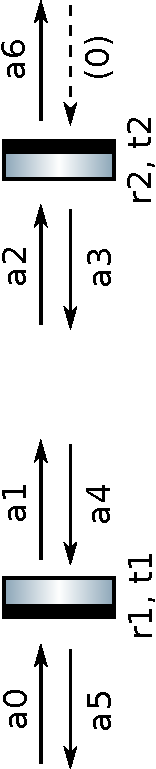
\includegraphics[height=0.4\textwidth, angle=-90]{figures/empty_cavity_amplitudes.pdf}
	\end{center}
	\caption{Labelled amplitudes for empty cavity matrix solution.}
	\label{fig:empty_cavity_amplitudes}
\end{figure*}

Consider an empty two-mirror cavity with reflectivities $r_1, r_2$ and transmitivities $t_1, t_2$. For simplicity we assume mirror 1 is lossless and mirror two is perfectly reflective $r_2 = 1, t_2 = 0$. Light $a_0(\Omega)$ is incident on mirror 1, where $a_0$ is a vector of the two quadratures in the frequency domain (see Section~\ref{sec:squeezing}). Let $a_j$ for $j = 1, \ldots, 6$ be similar and defined as in Fig.~\ref{fig:empty_cavity_amplitudes}. We use the mirror phase convention of no change on transmission and reflection from one of the sides and $\pi$ on reflection from the other side. The transmission and reflection matrices are therefore $R_i = r_i I,\; T_i = t_i I$, where $i = 1, 2$ and $I$ is the $2 \times 2$ identity matrix. Let the propagation matrix from one mirror to the other be $P$ which we construct later. Therefore, the amplitudes are related by
\begin{align*}
a_1 &= T_1 a_0 + R_1 a_4\\
a_2 &= P a_1\\
a_3 &= R_2 a_2 \\
a_4 &= P a_3\\
a_5 &= T_1 a_4 - R_1 a_0\\
a_6 &= T_2 a_2
\end{align*}
Solving the set of equations
\begin{align*}
a_4 &= P R_2 P (T_1 a_0 + R_1 a_4) \\
a_4 &= (I - P R_2 P R_1)^{-1} P R_2 P T_1 a_0 \\
a_5 &= \left(T_1 (I - P R_2 P R_1)^{-1} P R_2 P T_1 - R_1\right) a_0
\end{align*}
We get an expression for the reflected field off the cavity, $a_5$.


The propagation matrix $P$ across free space depends on the length and tuning of the space. Let the cavity be $D = L + \delta l$ long. Then the propagation across free space is
\begin{align*}
P(L, \delta l) &= \exp\left(i\frac{\Omega (L + \delta l)}{c}\right) \;\mathrm{Rot}\left(\frac{\omega_0 \delta l}{c}\right) \\
\mathrm{Rot}(\phi) &= \begin{bmatrix}
\cos(\phi) & -\sin(\phi)\\ 
\sin(\phi) & \cos(\phi)
\end{bmatrix}
\end{align*}
We assume that $\Omega \ll \omega_0$ and so $\frac{\Omega \delta l}{c} \ll 1$. Let the angular tuning be $\psi = \frac{\omega_0 \delta l}{c}$. Therefore $$P(L, \delta l) = \exp\left(i\frac{\Omega L}{c}\right) \;\mathrm{Rot}\left(\psi\right)$$

\subsubsection{Quadratures at the photodiodes}

To incorporate the squeezer we borrow the above solution but change the propagation matrix to
\begin{align*}
	\begin{gathered}
	\tilde{P}(L, \delta l, r, \phi) = P\left(\frac{L}{2}, \frac{\delta l}{2}\right) \mathrm{Sqz}(r, \phi) P\left(\frac{L}{2}, \frac{\delta l}{2}\right) \\
	\mathrm{Sqz}(r, \phi) = \begin{bmatrix}
	\cos(2 \phi) \sinh(r) + \cosh(r) & \sin(2\phi) \sinh(r)\\ 
	\sin(2\phi) \sinh(r) & -\cos(2 \phi) \sinh(r) + \cosh(r)
	\end{bmatrix}
	\end{gathered}
\end{align*}
Where $r = r_\mathrm{sqz}$ is the squeezer parameter (not in dB) and $\phi$ is the squeezer angle. Note that this means that the light gets squeezed from both directions by the squeezer. This is not what physically happens but is how \code{nle} is implemented, so for ease of comparison we choose this convention. Note that this is different to the directional squeezer in the analytics in Section~\ref{sec:aLIGOcomparison}.


Referring to Fig.~\ref{fig:squeezed_cavity}, let $n = a_0$ be the vacuum incident on the cavity, $a$ be the laser noise, and let the local oscillator itself be
$$A = A_0 \begin{bmatrix}
\cos(\theta)\\ 
\sin(\theta)
\end{bmatrix}$$
For homodyne angle $\theta$ and amplitude $A_0$. The field reflected off the cavity is
$$n_r = \left(t_1 (I - r_1 \tilde{P}^2)^{-1} \tilde{P}^2 t_1 - r_1 \right) n$$


For a 50/50 beamsplitter and negligible propagation lengths outside the cavity the fields (as quadrature vectors, frequency dependent) at the two photodiodes are therefore
\begin{align*}
b_1 &= \frac{1}{2^{1/2}} \left( n_r + A + a\right) \\
b_2 &= \frac{1}{2^{1/2}} \left( n_r - A - a\right)
\end{align*}

\subsubsection{Fourier spectrum of the time averaged intensity}

Consider the time average of the intensity at photodiode 1. Need to take inverse Fourier transform of frequency domain field, let tilde denote time domain. Note that depending on quadrature convention there may need to be a constant squared out the front of the intensity to fix the units, we later drop this constant anyway so I won’t write it. 
\begin{align*}
\tilde{b}_1 &= \begin{bmatrix}
\tilde{b}_{1,c}\\ 
\tilde{b}_{1,s}
\end{bmatrix} \\
\expect{\tilde{I}_1(t)} &= \expect{\abs{\tilde{b}_{1,c} \cos(\omega_0 t) + \tilde{b}_{1,s} \sin(\omega_0 t)}^2}
\end{align*}
Assuming that the time domain quadrature are Hermitian allows the absolute value squared to be expanded. Also assume that the quadratures are slowly changing with respect to $\omega_0$. Taking time averages we note $\expect{\cos(\omega_0 t) \sin(\omega_0 t)} = 0$ and $\expect{\cos^2} = \expect{\sin^2} = 1/2$. This leaves
$$\expect{\tilde{I}_1} = \frac{1}{2} \left( \tilde{b}_{1,c}^2 + \tilde{b}_{1,s}^2 \right)$$


Splitting the quadratures into a constant $B$ and a time varying part $\tilde{b}'$ with average zero and assuming that the time varying part is small with respect to the constant (this is true for the noise compared to the local oscillator). We expand the quadratures squared and drop the time varying part squared terms.
$$\expect{\tilde{I}_1} = \frac{1}{2} \left( B_{1,c}^2 + B_{1,s}^2 + 2 \left( B_{1,c} \tilde{b}_{1,c}' + B_{1,s} \tilde{b}_{1,s}' \right) \right)$$


Now taking Fourier transform to return to frequency domain, and dropping the (DC) constant term since we are only interested in the quantum noise. Recall that tildes indicated time domain, so we just drop them.
$$\expect{I_1} = B_{1,c} b_{1,c}' + B_{1,s} b_{1,s}'$$


We claim that these $B$ and $b'$ are the constant and frequency dependant parts of the original quadrature $b$. This amounts to $B$ being the local oscillator, e.g.\ $B_{1,c} = 1/2^{1/2} A_0 \cos(\theta)$, and $b'$ being the noise terms in $b$, i.e.\ $1/2^{1/2} (n_r \pm a)$. The homodyne intensity, $\mathrm{HomI}$, is then
$$\mathrm{HomI} = \expect{I_1 - I_2} = B_{1,c} b_{1,c}' + B_{1,s} b_{1,s}' - B_{2,c} b_{2,c}' - B_{2,s} b_{2,s}'$$


Substituting the quadratures at the photodiodes and simplifying reveals that the homodyne intensity doesn’t depend on $a$, the laser noise of the local oscillator, as expected. Let $n_c$ and $n_s$ be the quadratures of the original vacuum input $n$.
$$\mathrm{HomI} = \frac{A_0(g_1 n_c + g_2 n_s)}{g_3}$$
	
{\small
\begin{align*}
g_1 &= -\cosh ^2(r) e^{\frac{2 i L \Omega }{c}} \left(\cos (\theta ) \left(2 r_1^2+t_1^2\right) \cos (2 \psi )+t_1^2
   \sin (\theta ) \sin (2 \psi )\right) \\
   &-\cos (\theta ) \sinh ^2(r) \left(2 r_1^2+t_1^2\right) e^{\frac{2 i L \Omega
   }{c}}\\
   &-t_1^2 \cos (\theta ) \sinh (2 r) \cos (\psi ) \cos (2 \phi ) e^{\frac{2 i L \Omega }{c}}\\
   &-t_1^2 \sin (\theta )
   \sinh (2 r) \cos (\psi ) \sin (2 \phi ) e^{\frac{2 i L \Omega }{c}}\\
   &+r_1^3 \cos (\theta ) e^{\frac{4 i L \Omega
   }{c}}+r_1 t_1^2 \cos (\theta ) e^{\frac{4 i L \Omega }{c}}+r_1 \cos (\theta ) \\
g_2 &= \cosh ^2(r) e^{\frac{2 i L \Omega }{c}} \left(t_1^2 \cos (\theta ) \sin (2 \psi )-\sin (\theta ) \left(2
   r_1^2+t_1^2\right) \cos (2 \psi )\right)\\
   &+\sin (\theta ) \left(-\sinh ^2(r) (2 r_1^2+t_1^2\right)
   e^{\frac{2 i L \Omega }{c}}\\
   &+t_1^2 \sinh (2 r) \cos (\psi ) \cos (2 \phi ) e^{\frac{2 i L \Omega }{c}}+r_1^3
   e^{\frac{4 i L \Omega }{c}}+r_1 t_1^2 e^{\frac{4 i L \Omega }{c}}+r_1)\\
   &-4 t_1^2 \cos (\theta )
   \sinh (r) \cosh (r) \cos (\psi ) \sin (\phi ) \cos (\phi ) e^{\frac{2 i L \Omega }{c}} \\
g_3 &= 1 + r_1^2 e^{\frac{4 i L \Omega}{c}} - 2 e^{\frac{2 i L \Omega}{c}} r_1 \cos(2 \psi) \cosh(r)^2 - 2 e^{\frac{2 i L \Omega}{c}} \sinh(r)^2
\end{align*}
}

\subsubsection{PSD of the homodyne intensity}

Recall the definition of PSD from Section~\ref{sec:squeezing}, and noting that $S, \mathrm{HomI}, n$ should all have hats (\,$\hat{}$\,) but we drop them to reduce clutter.
$$S_\mathrm{HomI}(\Omega) 2 \pi \delta(\Omega - \Omega') = \langle0| \mathrm{HomI}(\Omega) \circ \mathrm{HomI}^\dagger(\Omega') |0\rangle$$

Assuming that the homodyne intensity is hermitian, and expanding out the symmetric products we get
\begin{align*}
S_\mathrm{HomI}(\Omega) 2 \pi \delta(\Omega - \Omega') &= \frac{A_0^2}{g_3(\Omega) g_3(\Omega')} \\
&\cdot \langle0| g_1(\Omega) g_1(\Omega') (n_c(\Omega) \circ n_c(\Omega'))\\
&+ g_2(\Omega) g_2(\Omega') (n_s(\Omega) \circ n_s(\Omega')) \\
&+ g_1(\Omega) g_2(\Omega') (n_c(\Omega) \circ n_s(\Omega')) \\
&+ g_2(\Omega) g_1(\Omega') (n_s(\Omega) \circ n_c(\Omega')) |0\rangle
\end{align*}


From pg.~38 of Ref.~\cite{Danilishin_2012}, for the quantum noise we have the following relations (the factor of $1/2$ is from the choice of using a double-sided PSD).
\begin{align*}
\langle0|n_c(\Omega) \circ n_c(\Omega')|0\rangle &= \frac{1}{2} 2 \pi \delta(\Omega - \Omega') \\
\langle0|n_s(\Omega) \circ n_s(\Omega')|0\rangle &= \frac{1}{2} 2 \pi \delta(\Omega - \Omega') \\
\langle0|n_c(\Omega) \circ n_s(\Omega')|0\rangle &= 0
\end{align*}

Substituting these relations in we arrive at the result, the PSD of the homodyne intensity. For plotting purposes we set $A_0 = 1$.
$$S_\mathrm{HomI}(\Omega) = \frac{A_0^2 \left( g_1(\Omega)^2 + g_2(\Omega)^2 \right)}{g_3(\Omega)^2}$$


%%%%%%%%%%%%%%%%%%%%%%%%%%%%%%%%%%%%%%%%%%
\nocite{*}
\bibliographystyle{myunsrt}
\bibliography{bib}


\end{document}
